\chapter{\TitreChapitreTrois}\label{chap:MiroirMobile}

\bfigh
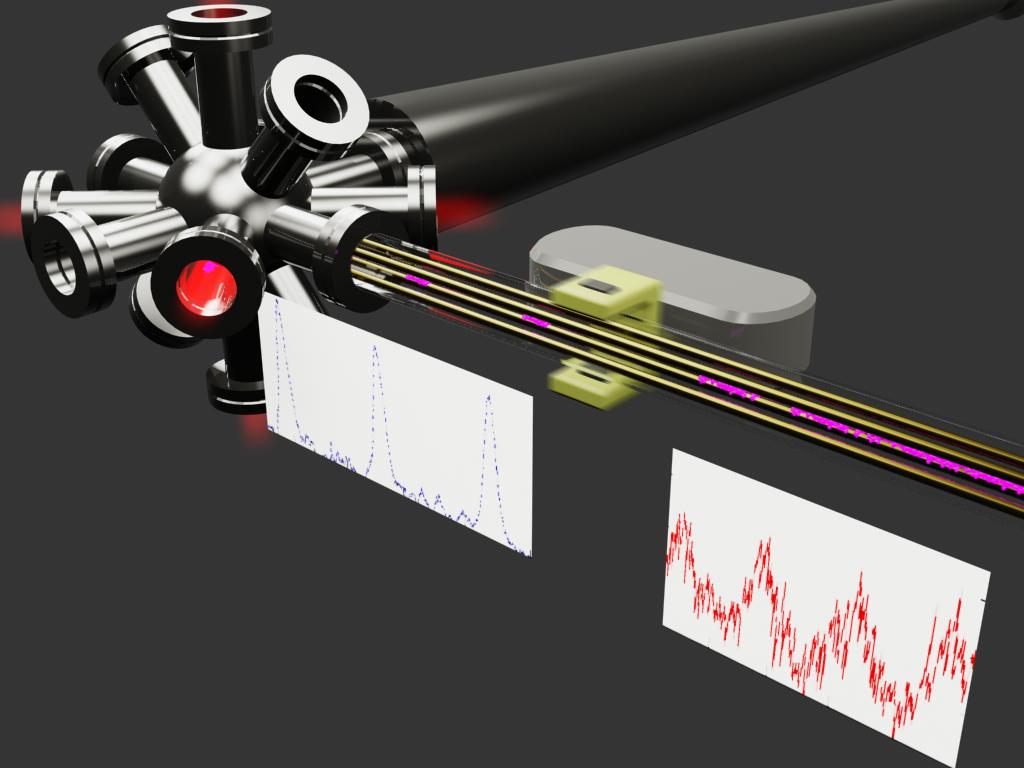
\includegraphics[width=\FigWidth]{P2/ChapitreMiroir}
{Représentation du \mimo utilisé sur notre \gm. Cette image a été publiée dans la section \nomofficiel{Highlight} de la revue EuroPhysics News afin d'illustrer les résultats de notre article~\cite{RWC06}.}%
% dont le résumé est fourni en annexe~\nref{annexe:Articles}.}%, \emph{A moving magnetic mirror to slow down a bunch of atoms}, joint en annexe.}
%\label{fig:MiroirEPN}
\efigh

\pagebreak

\minitoc

\section{Introduction}
Dans la première partie de ce manuscrit nous avons abordé le problème de la formation d'un \jatg, intense et lent. Rappelons-en ici les points importants qui nous seront utiles dans ce chapitre:
\begin{itemizel}
	\item l'injection pulsée de \pats dans le \gm permet d'obtenir des flux atomiques importants. L'optimisation de ce flux nous mène à l'utilisation de \emph{vitesses d'injection assez élevées} (typiquement \mps{1}).
	\item à l'inverse, nous avons tout intérêt à disposer d'un \jat (qui résulte du recouvrement des \pats) dont la \emph{vitesse moyenne est faible}, de manière à disposer d'un temps suffisant pour mener à bien le processus d'évaporation forcée. Corrélativement, pour un flux donné, un jet lent est linéiquement plus dense et chaque atome subit ainsi un nombre accru de collisions lors de sa propagation.
\end{itemizel}
Nous avons décrit une manière de concilier ces points, en ralentissant les atomes grâce à la mise en place d'une \secpent du \gm. Cette technique souffre cependant d'un défaut majeur : le ralentissement et la compression linéique du \jat s'accompagnent d'un échauffement et d'une mise hors d'\eqthdy de celui-ci.

\casse

Ce chapitre présente le ralentissement de \pats injectés dans le \gm par réflexion spéculaire sur un \mimamo. %Il est organisé de la manière suivante: 
Nous commencerons par souligne les limites liées à l'utilisation d'une \secpent comme moyen de ralentissement d'un \jat (voir l'annexe~\nref{annexe:SectionPentue}).
Après avoir introduit le principe de notre technique, et décrit la mise en \oe uvre expérimentale du \mima, nous présentons les résultats expérimentaux relatifs au ralentissement d'un \pat.
Finalement, nous discuterons nos résultats dans le contexte plus spécifique de l'utilisation de cette technique pour la formation d'un \jatuf et lent. 

La fin de ce chapitre sera consacrée à l'étude d'un point particulier de ce procédé de ralentissement. Celui-ci rend en effet possible l'obtention d'un jet ayant une \ddedp plus élevée que ce que nous obtiendrions grâce à l'utilisation d'une \secpent.
Ce point sera mis en regard du \thLi et nous amènera à considérer l'action du \mimo sur les \ps comme celle d'un \termetech{démon de Maxwell} (voir l'annexe~\nref{annexe:ThLi}).


\section{Limites du ralentissement par une \secpent}\label{sec:LimitePente}


Le fait de faire gravir une pente au \jat a bien pour effet de le ralentir, mais ceci se fait au prix d'un échauffement du jet, ou plus précisément, au prix d'une augmentation de la \dispvitlong. 

Le \thLi qui s'applique à tout système mécanique subissant une évolution hamiltonienne implique que, dans le cas d'un potentiel indépendant du temps, la \ddedp
reste constante le long de toute trajectoire. 
En d'autres termes, en suivant une particule dans son mouvement, la \fdd dans l'\edp qui l'environne reste constante. 
Rappelons que (d'après l'expression~\nref{eq:rhojetaxe} définie page \pageref{eq:rhojetaxe}) la \ddedp $\rhojetaxe$ suivant l'axe du \j suit la relation de proportionnalité%
\footnote{Toutes autres choses étant égales par ailleurs et en considérant le \pptlin, \cad avec le paramètre $\alpha = 0$.} :
\[
	\rhojetaxe \equiv \njetaxe \, \lambdaDB^3 
	\propto \frac{\flux}{\vjet\,T^\ttfrac{7}{2}} 
	\pointformule
\]
Or, pour un \j en régime stationnaire, le flux $\flux$ est constant lors de la propagation du jet. Le \thLi peut alors se traduire comme suit%
%\footnote{
%Nous supposons ici implicitement que le \jat est à l'\eqthdy de manière a pouvoir définir la température $T$.}% Il est cependant toujours possible de raisonner sur la dispersion de vitesse $\deltavjet$ du jet. On obtient alors $\vjet\,\deltavjet^\ttfrac{7}{4} = \const$.}
:
\begin{equation}
	\vjet\,T^\ttfrac{7}{2} = \const 
	\pointformule
	\label{eq:VT72Cste}
\end{equation}	
Ainsi, lors de sa propagation le long d'une \secpent, la vitesse moyenne du \jat va diminuer, alors que sa température va augmenter. 

\casse

%\Remarque%
\subsubsection{mise hors d'équilibre du \jat}
{
Précisons un point important relatif au fait que le jet gravit une pente.
En écrivant l'expression~\nref{eq:VT72Cste}, nous avons implicitement supposé que le jet est à l'\eqthdy de manière a pouvoir définir la température $T$. Il faut cependant remarquer le fait que la pente agit directement sur les degrés de liberté longitudinaux des atomes. L'annexe~\nref{annexe:SectionPentue} détail un calcul \ud montrant que la \dispvitlong du jet augmente au fur et à mesure que celui-ci progresse sur la \secpent. 
}



\section{Réflexion d'un \pat sur un \mimo}\label{sec:MethodeMiroir}

\subsection{Principe de la méthode}
Le principe mis en \oe uvre pour mener à bien le ralentissement des \pats dans le \gm rappelle qualitativement celui qu'un joueur de tennis utilise pour effectuer un \sotosay{amorti}. Lorsqu'une balle est soumise à un choc élastique avec un obstacle fixe (comme le terrain de tennis), le module de sa vitesse après l'impact reste inchangé, seule la direction de propagation de la balle est affectée par le rebond%
\footnote{On néglige tout effet dû à la rotation de la balle sur elle-même et aux frottements.}%
%
. \`A l'inverse, si la balle heurte un obstacle en mouvement (comme une raquette animée d'un mouvement de recul), la balle va pouvoir céder, ou absorber de l'énergie cinétique, et sa vitesse après le choc pourra être plus faible ou plus élevée%
\footnote{En réalité, au tennis, la raquette est presque immobile lors d'un amorti. Le véritable effet vient du fait que le joueur tient la raquette de manière relâchée, si bien que lors de l'impact, une partie ou la totalité de l'énergie cinétique de la balle est transmise à la raquette qui est alors projetée en arrière.}%
.


\subsubsection{Autres expériences utilisant ce principe}
Des expériences de physique atomique ont déjà exploité cette méthode afin de mener à bien le ralentissement d'atomes. L'obtention d'un faisceau ultra froid de neutrons a été rendue possible par réflexion spéculaire sur une surface de nickel en mouvement~\cite{SNS86}. Cette avancée fut à la source de beaucoup d'expériences dans les domaines de l'optique neutronique~\cite{WeK86,RaW01}.%
%} et de l'interférométrie avec des neutrons~\cite{


Dans un autre contexte, à l'université d'Austin (Texas), l'équipe du professeur Mark Raizen utilise des cristaux de silicium montés sur un rotor tournant à grande vitesse afin de décélérer par réflexion spéculaire un jet supersonique pulsé d'atomes d'hélium~\cite{LRB06}.
%, avec aussi pour but d'obtenir une source d'atome très intense pour les expériences d'optique atomique


\subsection{Modélisation simple de la collision avec un \mimo}
Afin de mieux comprendre la dynamique du problème, nous allons détailler dans cette section un modèle simple de la \colel d'un \pat avec une barrière en mouvement uniforme. Cette modélisation a été utilisée pour interpréter nos données expérimentales.%, dans le contexte de notre expérience de \pats guidés magnétiquement.

Nous nous intéressons à une modélisation unidimensionnelle du problème. De plus, nous négligeons les collisions entre atomes durant la propagation et la réflexion des \pats. Nous commençons donc par considérer la réflexion d'une seule particule. Une moyenne d'ensemble sera ensuite effectuée pour déduire l'évolution d'un \pat lors de la collision avec le \mimo.

\subsubsection{Collision d'une particule avec une barrière infinie de potentiel en mouvement}

Le problème le plus simple à envisager est celui de la collision élastique d'une seule particule sur une barrière infinie de potentiel. Un tel potentiel, qui réfléchit instantanément la particule incidente, joue le rôle d'un miroir, et sera désigné comme tel.
Nous utiliserons dans la suite les notations suivantes:
\begin{itemizel}
	\item l'origine des temps, $t=0$, est l'instant où la particule est injectée dans le \gm.
	\item $\Vmir$%
\nome{\Vmir}{Vitesse du \mimo}%
	, la vitesse du miroir sera prise indépendante du temps. Notamment, le mouvement de la barrière n'est pas affecté par la collision.
	\item la position du \mimo à l'instant initial est $\Zmirini \equiv \Zmir(t=0)$.%
\nome{\Zmir}{Position du \mimo à l'instant initial}% 
	\item $v(t)$ sera la vitesse (suivant l'axe du guide) de la particule dans le \reflab.
	\item la vitesse initiale (avant collision) de la particule est $\vatini$, sa vitesse finale (après collision) est $\vatfin$.
	\item $\tcol$ est l'instant de la collision.%
\nome{\tcol}{Instant de la collision d'un atome avec le \mimo}%
%
\end{itemizel}

\Remarque{\label{Rq:VitesseMiMoCste}
Nous considérons la vitesse du miroir comme étant constante.
Cette hypothèse est tout à fait valable dans le cas où la masse du \mimo (un objet macroscopique) est beaucoup plus importante que celle d'un atome. 
%Mais elle est aussi valable, même si les deux masses en jeu sont comparables, si la vitesse du miroir est asservie par un système extérieur.
}

\Resultat{
La figure~\nref{fig:MiroirChoc1Atome} permet d'analyser la dynamique du problème dans le \reflab et dans le \refmir. Après réflexion élastique sur le \mimo, la vitesse de la particule est:
%
\begin{equation}
	\vatfin \equiv v(t>\tcol) = 2 \Vmir - \vatini
	\pointformule
	\label{eq:Vreflexion}
\end{equation}
\finformule
}
\bfigh
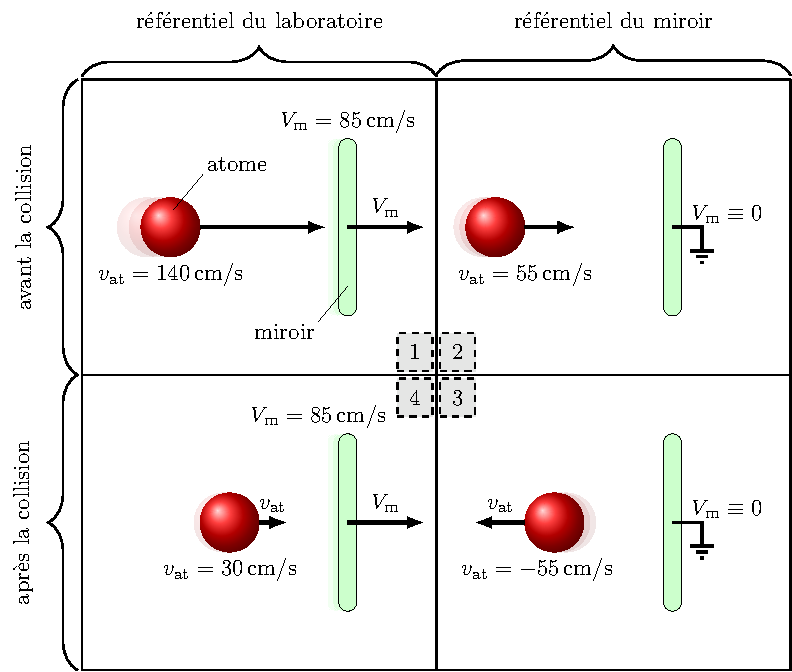
\includegraphics{P2/MiroirChoc1Atome}
\CaptionTocCaptionFig{Principe de la technique du ralentissement grâce à un miroir mobile}{ Principe de la technique du ralentissement grâce à un miroir mobile. Cette figure se lit dans le sens des aiguilles d'une montre en partant du cadran 1. Rappelons que la vitesse du \mimo est constante (voir remarque \vpageref{Rq:VitesseMiMoCste}).
\RemonteUnPeuFig
\vtop{\linewidth=\CaptionWidth %
\begin{description}
%
	\item[Cadran 1:] dans le \reflab, juste \emph{avant} la collision, la particule possède initialement une vitesse $\vatini \equiv v(t < \tcol)$ supérieure à la vitesse $\Vmir$ de la barrière. 
%	
	\item[Cadran 2:] dans le \refmir, juste \emph{avant} la collision, la particule possède une vitesse $\vatini-\Vmir$ > 0.
%	
	\item[Cadran 3:] dans le \refmir, juste \emph{après} la collision, qui se produit au temps $\tcol$, la particule possède une vitesse 
	$ - \left( \vatini-\Vmir \right) < 0$. La particule a été réfléchie.
%	
	\item[Cadran 4:] en nous replaçant dans le \reflab, juste \emph{après} la collision, nous calculons simplement la vitesse de la particule comme étant $ - \left( \vatini-\Vmir \right) + \Vmir$, soit :
\end{description}
	\[
	v_f \equiv v(t>\tcol) = 2 \Vmir - \vatini
	\pointformule
	\]
\RemonteUnPeuFig
\RemonteUnPeuFig
\RemonteUnPeuFig
\ApplicationNumerique{%
Pour des conditions typiques de nos expériences, il est ainsi possible de ralentir un atome de \cmps{140} à \cmps{30} grâce à un \mimo ayant une vitesse de \cmps{85}. L'énergie cinétique longitudinale de la particule a donc été réduite de $95\%$ (voir la section~\nref{sec:ResultatPaquetUnique}).}
}}
\label{fig:MiroirChoc1Atome}
\efigh

\subsubsection{Modélisation d'un \pat}

Pour un \pat dont l'extension longitudinale moyenne au moment de la collision est $\Delta_z$, l'instant $\tcol$ est différent pour chaque atome du paquet, et la réflexion s'étend donc sur un laps de temps de l'ordre de $\Tcol \equiv \tfrac{\Delta_z}{\MoyenneBraKet{\vatini}-\Vmir}$.
\nome{\Tcol}{Durée typique de la collision d'un \p avec le \mimo}%
%
  
Une description rigoureuse de la dynamique d'évolution  du \pat lors de sa réflexion devrait faire intervenir l'effet éventuel des collisions entre atomes. Nous pouvons cependant les négliger à partir du moment où $\Tcol$ est petit devant le temps moyen entre deux collisions inter-atomiques. Dans nos expériences cette hypothèse est bien vérifiée%
%\footnote{La densité des \pats dont il est question dans cette partie est effectivement assez faible pour pouvoir négliger les collisions durant la réflexion.}%
.

\`A l'instant $t=0$, le nuage est modélisé par une distribution spatiale ponctuelle, mais gaussienne en vitesse, \cad que la taille initiale du \pat est négligée. Cette modélisation n'a de sens que si la \dispvitlong conduit à un étalement du nuage au moment de la collision jusqu'à une taille grande devant la taille initiale réelle du \pat. Nous verrons plus loin que cette hypothèse est expérimentalement raisonnable (voir la section~\nref{sec:ResultatPaquetUnique}). Nous considérons donc la \fdd initiale dans l'\edpup:

\begin{equation}
	f_i(z,v) \equiv C \Expo{-\frac{m}{2\,\kb\,\Tlongini} 
	\left( v - \vinj \right)^2} \times \Dirac{z}
	\virguleformule
	\label{eq:fiPaquet}
\end{equation}
où $\vinj$ est la vitesse moyenne du \pat au moment de l'injection dans le \gm et $C$ est une constante de normalisation.
\nome{\vinj}{Vitesse moyenne du \pat au moment de l'injection}%
%


\subsection{Réflexion d'un \pat}
\subsubsection{Propagation libre du \pat}
Dès l'injection du \pat dans le \gm, la \dispvitlong conduit à un étalement du paquet. Nous faisons l'hypothèse que les atomes du paquet n'interagissent pas entre eux. Par suite, chaque atome se propage librement à vitesse constante et nous pouvons alors facilement écrire la \fdd du \pat à chaque instant avant la collision:
\begin{align}
	f(z,v,t) 
	&= 
%	\Integrale{
%	\Integrale{
\iint {{
	f_i(z_0,\vini)\,\Dirac{z - (z_0 + \vini t)}\,\Dirac{\vini - v}
	}{\ddint \vini}}{\ddint z_0} \nonumber \\
	&=
%	\Integrale{
%	\Integrale{
\iint {{
	C\,\Expo{-\frac{m}{2\,\kb\,\Tlongini} \,
	\left( \vini - \vinj \right)^2}\,\Dirac{z_0}\,\Dirac{z - (z_0 + \vini\,t)}\,\Dirac{\vini - v}
	}{\ddint \vini}}{\ddint z_0}
	\virguleformule
\end{align}
où l'on reconnaît, dans les fonctions $\Dirac{}$ de Dirac, la traduction d'un mouvement rectiligne uniforme.
%
\Resultat{
Nous obtenons donc l'expression de la \fdd du nuage (initialement ponctuel) dans le \gm avant la collision avec le \mimo:
\begin{equation}
	f(z,v,t) = C\,\Expo{-\frac{m}{2\,\kb\,\Tlongini} 
	\left( v - \vinj \right)^2}\,\Dirac{z - v\,t}
	\virguleformule
	\label{eq:ftPaquetAvantCol}
\end{equation}
\finformule
}
L'expression~\nref{eq:ftPaquetAvantCol} s'interprète de la manière suivante: 
\begin{itemize}
	\item on retrouve bien la même distribution en vitesse puisque le \pat se propage librement (c'est la distribution gaussienne),
	\item mais le terme $\Dirac{z - v\,t}$ traduit mathématiquement les corrélations position-vitesse qui se développent au cours de la propagation. Les atomes \sotosay{rapides} se retrouvent \sotosay{à l'avant} du nuage (\cad vers les $z$ élevés), alors que les atomes \sotosay{lents} restent à \sotosay{l'arrière} du nuage (vers les $z$ faibles).
\end{itemize}

\Resultat{
La \dat linéique $n(z,t)$ se déduit par une intégration sur la variable de vitesse $v$:
\begin{equation}
	n(z,t) \equiv \Integrale{f(z,u,t)}{\ddint u} 
	= C \, \Expo{-\frac{m}{2 \, \kb \, \Tlongini} 
	\, \left( \dfrac{z}{t} - \vinj \right)^2}
	\pointformule
	\label{eq:ntPaquetAvantCol}
\end{equation}%
\finformule
}


\casse


\subsubsection{Réflexion du \pat}\label{sec:ftPaquetReflechi}

Pour chacun des atomes d'un paquet décrit par la distribution~\nref{eq:fiPaquet}, l'instant $\tcol$ de la collision avec le \mimo correspond au temps qu'il a fallu pour que cet atome (dont la vitesse initiale est $\vini$) \sotosay{rattrape} le miroir, qui à l'instant $t=0$ se trouve en $z=\Zmirini$ et dont la vitesse est $\Vmir < \vini$:
\begin{equation}
	\tcol(\vini) = \frac{\Zmirini}{\vini - \Vmir}
	\pointformule
	\label{eq:tcol}
\end{equation}

\noindent
La figure~\nref{fig:TcolAtomeV0} représente, dans l'\edpup, les trajectoires de quelques atomes de la distribution~\nref{eq:fiPaquet}.

\bfigs
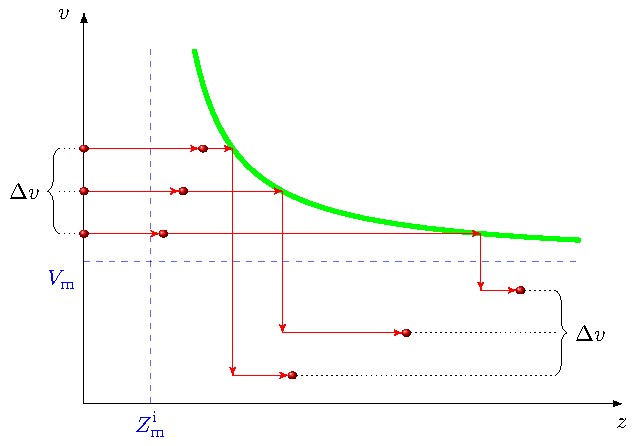
\includegraphics{P2/TcolAtomeV0}
\CaptionFigs{Représentation de la collision dans l'\edpup ($z$,$v$) pour quelques trajectoires atomiques correspondant à la distribution~\nref{eq:fiPaquet}. \\
À l'instant initial, tous les atomes sont en $z=0$, mais ont des vitesses initiales $\vini$ différentes. Les lignes pointillées représentent la vitesse $\Vmir$ et la position initiale est $\Zmirini$ du \mimo. La courbe hyperbolique représente les points de l'\edp où un atome de vitesse initiale $\vini$ rencontre le miroir. \\
Les cercles représentent quelques atomes à l'instant initial, à un instant \emph{avant} la collision du \pat, puis \emph{après} la collision.\\
$\Delta v$ désigne la dispersion de vitesse pour les trois atomes considérés dans cet exemple. La vitesse d'un atome après réflexion est symétrique de sa vitesse initiale par rapport à $\Vmir$. Ainsi, on constate que la réflexion, tout en ralentissant le paquet, conserve la dispersion de vitesses $\Delta v$, contrairement à l'effet d'une pente.}
\label{fig:TcolAtomeV0}
\efig

\noindent
Ainsi, en tenant compte de l'équation~\nref{eq:Vreflexion}, la vitesse au cours du temps $\vat(t)$ de cet atome s'écrit
\begin{equation}
	\vat(t; \vini) = 
	%\ArriveeHiglightColorMath{blue}
	{\vini\,\Heaviside{\tcol(\vini)-t}}
	+ 
	%\ArriveeHiglightColorMath{red}
	{(2\, \Vmir - \vini) \Heaviside{t-\tcol(\vini)}}
	\virguleformule
	\label{eq:vtAtomeReflexion}
\end{equation}
où les vitesses de la particule %\DepartHighlightColor{blue}
{avant} et %\DepartHighlightColor{red}
{après} la collision apparaissent clairement, $\Heaviside{}$ est la \termetech{fonction de Heaviside}. 
Aussi, nous connaissons la position $\zat(t)$ de cet atome en intégrant l'équation~\nref{eq:vtAtomeReflexion}:
%\MakeFlecheHighlightColor{blue}%
%\MakeFlecheHighlightColor{red}%
\begin{equation}
	\zat(t; \vini) \equiv \IntegraleBornes{\vat(t'; \vini)}{\ddint t'}{0}{t} = \vini t - 2\,(\vini-\Vmir)\,(t-\tcol(\vini)) \Heaviside{t-\tcol(\vini)}
	\pointformule
	\label{eq:ztAtomeReflexion}
\end{equation}
L'évolution de la fonction de distribution du \pat s'établit en utilisant les équations~\nref{eq:fiPaquet} et~\nref{eq:tcol} à~\nref{eq:ztAtomeReflexion}. 
%
\EnFaitNon
{

\begin{align}
	f(z,v,t) 
	=& 
	\iint
	%\DepartHighlightColorMath{blue}
	{
	f_i(z_0,\vini)
	}	
	%\DepartHighlightColorMath{red}
	{
	\Dirac{z - \zat(t)}
	}	
	%\DepartHighlightColorMath{green}
	{
	\Dirac{v - \vat(t)}
	}
	\ddint \vini \ddint z_0 \nonumber\\
	=& 
	\iint
	%\ArriveeHiglightColorMath{blue}
	{
	C \Expo{-\frac{m}{2\,\kb\,\Tlongini} 
	\left( \vini - \vinj \right)^2}\Dirac{z_0}
	}
	\nonumber\\
%%%%%%%%%%%%%%%%%%%%%%%%%%%%%%%%%%%%%%%%%%%%%%%%%%%%%%%%%%%%%%%%%%%%%%%%%%%%%%%%%%%%%%%%%%%%%%%%%%%%%%%%%%%%%%%%%%%%%%%%%%%%%%%%%%%%%%%%
	&	\;\;\;\;\;\;\;\;\;\; 
	%\ArriveeHiglightColorMath{red}
	{\DIRAC{z - \left( \vini t - 2(\vini-\Vmir)\left(t - \frac{\Zmirini}{\vini - \Vmir}\right) \Heaviside{t -  \frac{\Zmirini}{\vini - \Vmir}} \right)} 
	}
	\nonumber\\
%%%%%%%%%%%%%%%%%%%%%%%%%%%%%%%%%%%%%%%%%%%%%%%%%%%%%%%%%%%%%%%%%%%%%%%%%%%%%%%%%%%%%%%%%%%%%%%%%%%%%%%%%%%%%%%%%%%%%%%%%%%%%%%%%%%%%%%%
	&	\;\;\;\;\;\;\;\;\;\; 
	%\ArriveeHiglightColorMath{green}
	{\DIRAC{v - \left( \vini \Heaviside{\frac{\Zmirini}{\vini - \Vmir} - t} + (2 \Vmir - \vini) \Heaviside{t - \frac{\Zmirini}{\vini - \Vmir}} \right)}
	}
	\nonumber\\
	&	\;\;\;\;\;\;\;\;\;\; \ddint \vini \ddint z_0
	\pointformule
	\label{eq:ftPaquet}
\end{align}
%\MakeFlecheHighlightColor{blue}\MakeFlecheHighlightColor{red}\MakeFlecheHighlightColor{green}
%Dans cette égalité, les différents termes de l'intégrale sont repérés par des couleurs lors de leur développement. 
On note que l'intégration suivant la variable $z_0$ est immédiate du fait de la présence du terme $\Dirac{z_0}$, et nous effectuons le remplacement directement.
Cette équation~\nref{eq:ftPaquet} ne semble pas simple à intégrer dans la mesure où les termes de Dirac contiennent des fonctions de Heaviside et que la vitesse $\vini$ y apparaît plusieurs fois, notamment au dénominateur. 

En revanche, on remarque que la condition sur le temps $t$ pour qu'un atome ayant une vitesse initiale $\vini$ donnée ait subi la collision avec le \mimo et qui s'écrit:
\[
	t \geq \tcol(\vini) = \frac{\Zmirini}{\vini - \Vmir} 
	\virguleformule
\]
peut se traduire (d'après l'équation~\nref{eq:tcol}) de manière équivalente en une condition sur la vitesse initiale $\vini$ d'un atome, traduisant le fait que ce dernier \emph{aura} subi la collision à un temps $t$ donné:
\begin{equation}
	\vini \geq \vinicol(t) \equiv \Vmir + \frac{\Zmirini}{t} 
	\pointformule
	\label{eq:vinicolt}
\end{equation}
$\vinicol(t)$ est, pour ainsi dire, \sotosay{la vitesse initiale dont un atome a besoin afin de subir une collision à l'instant $t$ choisi}.


Grâce à cette formulation, on peut ré-écrire l'argument des fonctions de Heaviside des équations~\nref{eq:vtAtomeReflexion} et~\nref{eq:ztAtomeReflexion} de manière à exprimer l'équation~\nref{eq:ftPaquet} sous la forme:
\begin{align}
	f(z,v,t)
	=&
	\int
%%%%%%%%%%%%%%%%%%%%%%%%%%%%%%%%%%%%%%%%%%%%%%%%%%%%%%%%%%%%%%%%%%%%%%%%%%%%%%%%%%%%%%%%%%%%%%%%%%%%%%%%%%%%%%%%%%%%%%%%%%%%%%%%%%%%%%%%
	%\ArriveeHiglightColorMath{blue}
	{
	C \Expo{-\frac{m}{2\,\kb\,\Tlongini} 
	\left( \vini - \vinj \right)^2}
	}
	\nonumber\\	%%%%%%%%%%%%%%%%%%%%%%%%%%%%%%%%%%%%%%%%%%%%%%%%%%%%%%%%%%%%%%%%%%%%%%%%%%%%%%%%%%%%%%%%%%%%%%%%%%%%%%%%%%%%%%%%%%%%%%%%%%%%%%%%%%%%%%%%
	&	\;\;\;\;\; 
	%\ArriveeHiglightColorMath{red}
	{\DIRAC{z - \vini t + 2(\vini-\Vmir)\left(t - \frac{\Zmirini}{\vini - \Vmir}\right) \Heaviside{\vini - \vinicol(t)} }
	}
	\nonumber\\
%%%%%%%%%%%%%%%%%%%%%%%%%%%%%%%%%%%%%%%%%%%%%%%%%%%%%%%%%%%%%%%%%%%%%%%%%%%%%%%%%%%%%%%%%%%%%%%%%%%%%%%%%%%%%%%%%%%%%%%%%%%%%%%%%%%%%%%%
	&	\;\;\;\;\;
	%\ArriveeHiglightColorMath{green}
	{\DIRAC{v - \vini \Heaviside{\vinicol(t) - \vini} - (2 \Vmir - \vini) \Heaviside{\vini - \vinicol(t)}}
	}
	\nonumber\\
	&	\;\;\;\;\; \ddint \vini \nonumber
	\virguleformule
\end{align}
qui se coupe naturellement en deux en intégrant de $-\infty$ à $\vinicol(t)$, puis de $\vinicol(t)$ à $+\infty$. Ceci simplifie les fonctions de Heaviside qui valent sur ces domaines soit $0$, soit $1$:
\begin{align}
	f(z,v,t)	=&
	\IntegraleBornes{
	C \Expo{-\frac{m}{2\,\kb\,\Tlongini} \left( \vini - \vinj \right)^2}
	\Dirac{z - \vini t}
	\Dirac{v - \vini}
%	}
	}{\ddint \vini}{-\infty}{\vinicol(t)} \nonumber \\
	+&\IntegraleBornes{
	C \Expo{-\frac{m}{2\,\kb\,\Tlongini} \left( \vini - \vinj \right)^2}
	\Dirac{z - t( 2\Vmir-\vini) - 2 \Zmirini}
	\Dirac{\vini + v - 2 \Vmir}
%	}
	}{\ddint \vini}{\vinicol(t)}{+\infty} \nonumber
	\virguleformule
%	\label{eq:ftPaquetSimple}
\end{align}

}
%
%\Resultat
{
%En conclusion, nous pouvons établir 
On peut ainsi calculer
la \fdd d'un \pat initialement ponctuel de \templong $\Tlongini$ injecté à l'instant initial à une vitesse moyenne $\vinj$ en direction d'une barrière infinie de potentiel ayant une vitesse $\Vmir$ et une avance $\Zmirini$ à l'instant initial:
\begin{align}
	f(z,v,t)	=&%
	C \Expo{-\frac{m}{2\,\kb\,\Tlongini} \left( v - \vinj \right)^2}
	\Dirac{v - \frac{z}{t}}
	\Heaviside{\Vmir + \frac{\Zmirini}{t} - v}	\nonumber \\
	+&%
	C \Expo{-\frac{m}{2\,\kb\,\Tlongini} \left( v - 2 \Vmir + \vinj \right)^2}
	\Dirac{v - \frac{z-2\Zmirini}{t}}
	\Heaviside{\Vmir - \frac{\Zmirini}{t} - v}
	\pointformule
	\label{eq:ftPaquetResultat}
\end{align}
On distingue bien ici les deux termes correspondant:
\begin{itemizel}
	\item au nuage initialement injecté dans le guide magnétique (voir l'équation~\nref{eq:ftPaquetAvantCol}) qui intervient aux temps courts (avant la collision du nuage avec le \mimo).
	\item au nuage réfléchi, dont la vitesse moyenne est $2\,\Vmir-\vinj$ et qui intervient aux temps longs (après la collision). On remarque aussi dans ce terme, que la \templong n'a pas été modifiée lors de la collision. 
\end{itemizel}
}
Le fait de ne pas modifier la \dispvitlong du \pat est une propriété remarquable qui distingue la \techmimo par rapport à l'utilisation d'une \secpent. Ce point est discuté dans la section~\nref{sec:MiroirVioleLiouville}

%\Intuition{Une manière simple de se convaincre que les propriétés du \pat ne sont pas modifiées par la réflexion sur le \mimo peut se présenter sous cette forme, par analogie avec l'optique newtonienne:
%
%\emph{après} la collision, nous obtenons un \pat qui est tout simplement \emph{l'image} du paquet initial par réflexion dans un miroir, et dont les propriétés sont identiques. 
%}


\subsection{Évolution de la densité atomique dans le \gm}

Comme nous l'avons précisé dans le chapitre~\nref{chap:JetAtomique} (section~\nref{sec:MesureJat}), la grandeur qui nous est expérimentalement accessible par la mesure est la \datlin $n(z,t)$ dans le \gm. 
\Resultat{
Celle-ci s'obtient par intégration de l'équation~\nref{eq:ftPaquetResultat} par rapport à la variable $v$:
\begin{align}
	n(z,t) & \equiv	\Integrale{f(z,v,t)}{\ddint v} \nonumber \\
	& =C \left[ \Expo{-\frac{m}{2\,\kb\,\Tlongini} \left( \frac{z}{t} - \vinj \right)^2}
	\right.
	\nonumber \\
	& \qquad +
	\left.
	\Expo{-\frac{m}{2\,\kb\,\Tlongini} \left( \frac{z-2\Zmirini}{t} - 2 \Vmir + \vinj \right)^2} \right] \Heaviside{t\,\Vmir + \Zmirini - z}
	\pointformule
	\label{eq:NtPaquetResultat}
\end{align}
\finformule
}

\casse

\noindent
L'expression~\nref{eq:NtPaquetResultat} s'interprète en remarquant que La \dat est donnée par la somme des contributions de deux nuages se propageant en sens inverse:
\begin{itemize}
	\item le premier terme de la somme entre parenthèses correspond au nuage initial lancé dans le guide.
	\item le second terme correspond au nuage symétrique du premier par rapport au \mimo dont l'équation du mouvement est $\Zmirini + \Vmir\,t$.
	\item le terme $\Heaviside{\cdots}$ de Heaviside traduit mathématiquement le fait qu'aucun atome n'est en fait passé de l'autre coté du \mimo ($z > \Zmirini + t\,\Vmir$).
\end{itemize}


\noindent
La figure~\nref{fig:NtPaquetResultat} donne une représentation de l'expression~\nref{eq:NtPaquetResultat} en fonction de $z$ à des instants $t$ caractéristiques: \emph{avant}, \emph{pendant}, et \emph{après} la collision du \pat avec le \mimo.%

\bfigs
%
\ifthenelse{\NoAnimationsInFigures > 0}{%
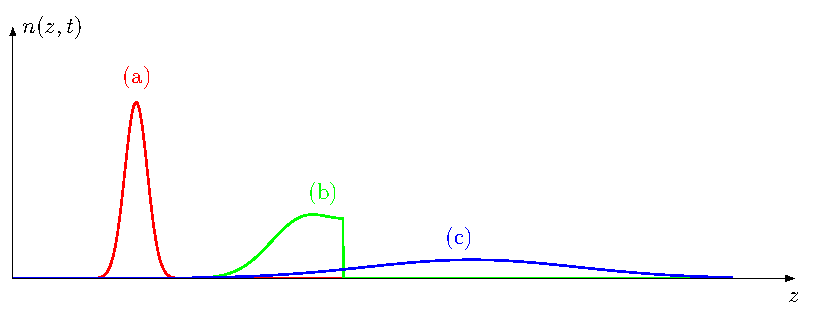
\includegraphics{P2/NtPaquetResultatAnimate_1}%
}{%
\animategraphics[poster=last]{10}{images/P2/NtPaquetResultatAnimate}{}{}%
}
\CaptionFigs{\AnimateOnline Représentation de la \datlin $n(z,t)$ donnée par l'expression~\nref{eq:NtPaquetResultat} en fonction de $z$ pour différents instants : (a) avant, (b) pendant, et (c) après la collision.}
\label{fig:NtPaquetResultat}
\efig

%
%\subsection{Réflexion élastique sur une barrière harmonique en mouvement}\label{sec:BarriereHarmonique}
%L'étude d'une barrière de potentiel non-infini, \cad qui ne se comporte pas comme un miroir vis a vis des atomes est plus délicate. En effet, la relation~\nref{eq:Vreflexion} reste valable, mais l'équation~\nref{eq:vtAtomeReflexion} n'est plus juste dans la mesure où les atomes ne rebondissent plus instantanément. Le temps qu'un atome va mettre à être réfléchi (au sens de l'équation~\nref{eq:Vreflexion}) va en général dépendre de sa vitesse. 
%Il existe cependant une autre forme de potentiel qui donne un résultat simple: Un potentiel en forme de demi-parabole. En rencontrant un tel potentiel, toutes les particules mettent le même temps à être réfléchies puisque la (demi-)période d'oscillation est indépendante de la vitesse d'arrivée des atomes. Ainsi, tout ce passe avec une barrière à forme harmonique comme avec une barrière infinie, mais avec un décalage temporel d'une demi-période d'oscillation.


\section{Mise en \oe uvre expérimentale}\label{sec:MiroirMiseEnOeuvre}

%Comme évoquer plus haut, cette méthode repose sur l'utilisation d'un potentiel dépendant du temps, prenant la forme ici d'un \mimo. Il existe différentes manières expérimentales pour mettre en \oe uvre cette technique.
%Certaines équipe utilise des courant alternés dans des bobine afin de mettre en mouvement des atomes. da.................

\subsection{Un \mima à aimants permanents}

\subsubsection{Différentes manières de réfléchir des atomes}
La réflexion d'atomes sur \mimo a déjà été étudiée dans le contexte des atomes ultra-froids. L'utilisation d'ondes lumineuses évanescentes se propageant à la surface d'un prisme, et dont l'intensité était modulée dans le temps, permit la manipulation d'atomes pour l'optique atomique: focalisation de trajectoires atomiques, formation d'images multiples d'un point source et modulation de la phase d'onde de De Broglie~\cite{SSD95,ASD96}.

La mise en \oe uvre d'un \mima repose sur l'interaction Zeeman entre un \chm inhomogène et le moment dipolaire magnétique des atomes. 
Des miroirs magnétiques pour l'optique atomique ont été réalisés de manières variées, en utilisant des arrangements d'aimants permanents~\cite{SMR96}, des micro-électro-aimants~\cite{JDT98, DZL99}, ou encore divers supports magnétiques (tels que de des disquettes informatiques~\cite{HBR97}, des bandes vidéo~\cite{RHH00}).  
%L'équipe de Tilma Esslinger en Allemagne a montré qu'il était possible de manipuler, sur ce principe, des ondes cohérentes de matières (extraites d'un \bec d'atome de \Rb)~\cite{BKG01}.

\casse

\subsubsection{Produire une \bapot dans le \gm}

Nous allons maintenant nous intéresser à la réalisation expérimentale d'une barrière de potentiel magnétique sur l'axe $z$ de notre guide. La mise en mouvement de cette barrière sera traitée dans la \autoref{sec:MiroirMiseEnMouvement}.

%Dans le \gm de notre \setup, les atomes se propagent librement suivant la direction $z$. 
%La réalisation d'un \mima suivant l'axe de propagation des atomes repose sur le fait que, dans nos conditions expérimentales, le potentiel effectivement ressenti par les atomes est proportionnel au module du \chm\footnote{Le potentiel ressenti par les atomes est proportionnel au module du \chm seulement dans l'hypothèse d'une évolution adiabatique des atomes au sein du \chm, \cad que les moments magnétiques des atomes doivent rester alignés avec les ligne de champ. Cette hypothèse est valide pour toute nos expériences.} et dépend donc de la composante longitudinale du \chm. 
Nous avons choisi d'utiliser des aimants permanents afin de moduler la valeur du \chm longitudinal $\Bpara\,\Vecteur{e_z}$ sur l'axe du guide. En effet, nous avons vu dans la section~\nref{sec:ConfigMagnetiqueGuide} que le potentiel auquel sont soumis les atomes dans le guide dépend, entre autres choses, de la composante longitudinale du \chm. Ainsi, une valeur localement élevée du champ $\Bpara$ va avoir pour effet de repousser les atomes de \Rb préparés dans l'état $\EtatSFmF{1}{-1}$.
Nous pourrons donc réflechir un atome dans le guide si la \bapot magnétique possède une hauteur suffisante (\cad supérieure à l'énergie cinétique longitudinale de l'atome).

\EnFaitNon{
Le \chm longitudinal dont il est question ici peut etre produit de différentes manières:
\begin{itemize}
	\item Bobine suivant l'axe du \gm: Cette technique est simple à mettre en \oe uvre mais la mise en mouvement d'une bobine enroulée autour du guide parait délicate, notamment s'il s'agit de faire se mouvoir ce montage de manière répétée.
	\item Paire de bobines placées de part et d'autre du guide:] Ceci rappelle la configuration utilisée pour l'évaporation du \jat sur une céramique du chapitre~\nref{chap:Ceramique} dans leque les bobines étaient placées en configuration Helmholtz, produisant un fort champ transverse. Afin de créer un champ longitudinal sur l'axe du \gm, les bobines doivent être placées en configuration anti-Helmholtz. Le champs transverses des deux bobines s'annulent ainsi sur l'axe du guide. 
	\item Paire d'aimants permanents: Encore en rapport avec le chapitre mentionné précedemment dans lequel nous avons utilisé une paire d'aimants permanent créant un fort \chm transverse. Cette fois-ci, les aimants sont placés en vis-à-vis avec des aimentations opposées de manière à produire un champ longitudinal sur l'axe du \gm. 
\end{itemize}

C'est cette dernière solution qui à été retenue car elle ne nécessite pas d'apport de courant et se présente sous la forme d'un montage léger et facile à mettre en mouvement. 
}


\subsection{Disposition des aimants autour du \gm}
%Nous décrivons ici la configuration géométrique utilisée pour le positionnement des aimants.

%\Remarque
{
\subsubsection{Disposition symétrique des aimants}
Si nous désirons moduler spatialement la composante longitudinale $\Bpara$ du \chm sur l'axe du guide, il est en revanche très important de ne pas générer de composantes transverses. En effet, nous avons vu au chapitre~\nref{chap:Ceramique} que moduler le champ transverse a pour effet de dévier latéralement la trajectoire des atomes. Ceci conduit à une élimination de certains atomes si cette déviation se fait au niveau d'une pièce en céramique (voir la \autoref{sec:ResultatVariationFlux}).

Afin de ne pas avoir de composantes transverses du \chm au niveau de l'axe du guide, celui-ci doit être un \emph{axe de symétrie} pour l'alimentation, \cad qu'il faudra disposer les aimants de manière symétrique par rapport au guide, avec leur aimantation deux à deux opposées. Dans notre cas, l'aimantation de chaque aimant pointe vers le guide.
La configuration choisie ainsi que l'allure de la \bapot produite suivant l'axe du \gm sont représentées sur la figure \ref{fig:AimantPaireChampLong}.
}
\bfighs
\subfloat[]{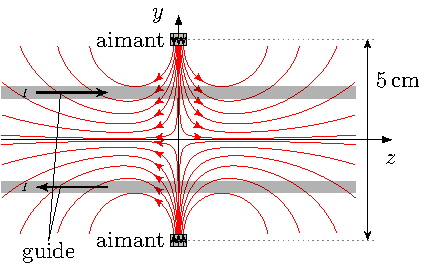
\includegraphics{P2/AimantPaireChampLong}}
\subfloat[]{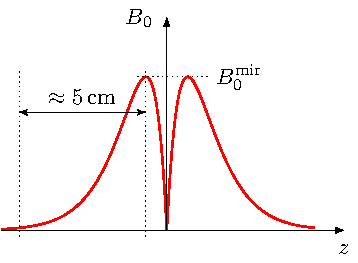
\includegraphics{P2/AimantPaireChampLongAxe}}
\CaptionFigs{
(a): disposition des aimants autour de l'axe $z$ du \gm et représentation de quelques lignes de \chm des aimants. Une configuration symétrique de l'aimantation par rapport à l'axe $z$ permet de produire un champ purement longitudinal sur cet axe. L'espacement entre les aimants est d'environ \cm{5}.
(b): allure du module du \chm sur l'axe $z$ du guide. Pour des atomes préparés dans l'état $\EtatSFmF{1}{-1}$, cela correspond à une \bapot dont la hauteur est déterminée par la valeur maximale $\Bparamir$. L'extension longitudinale de cette barrière est d'environ \cm{5}.
}
\label{fig:AimantPaireChampLong}
\efigh

\casse

Les aimants utilisés sont les mêmes que ceux qui ont servi pour l'évaporation sur une céramique (chapitre~\nref{chap:Ceramique}) et sont décrits dans l'annexe~\nref{annexe:ModelisationAimants}.
Ils sont placés sur un support en polystyrène %
\footnote{L'utilisation d'un matériau léger pour confectionner le support du \mimo est justifiée dans la \autoref{sec:MiroirMiseEnMouvement}.} %
ayant la forme d'un \enquote{U}.
La figure~\nref{fig:MiroirMontageAimant} représente ce montage et le positionnement de celui-ci autour du \gm. 
\bfighs
\subfloat[]{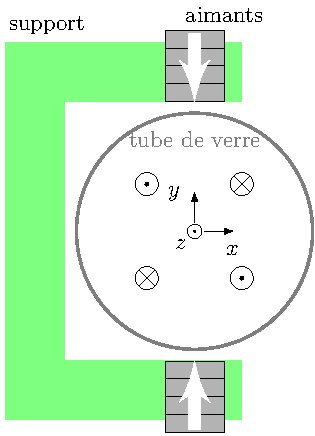
\includegraphics{P2/MiroirMontageAimant}}\quad
\subfloat[]{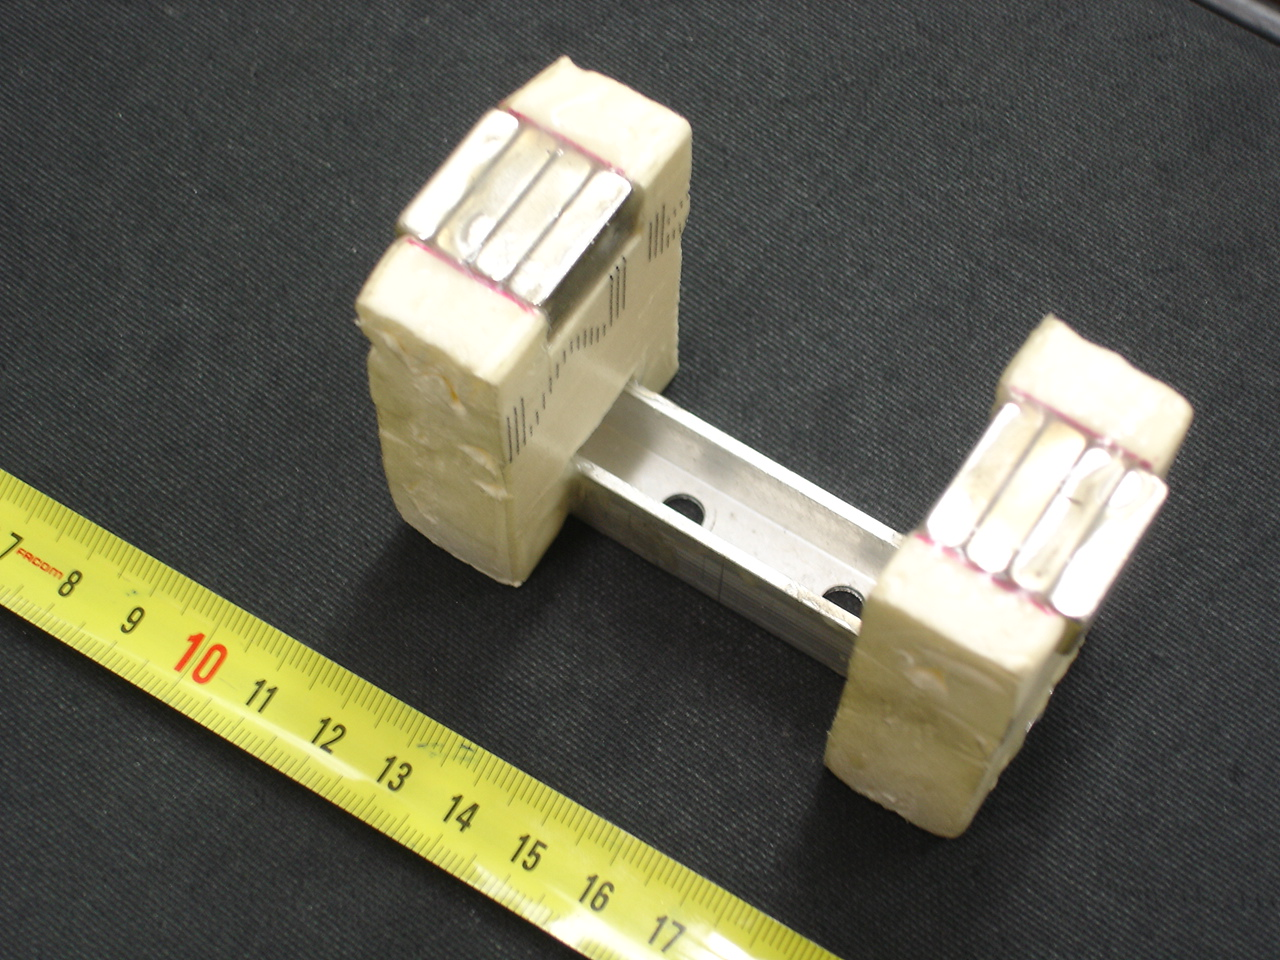
\includegraphics[height = 7cm]{P2/MiroirMontageAimantPhoto}}
\CaptionFigs{(a): Vue schématique en coupe du \mima en place autour du guide. L'utilisation de plusieurs aimants de chaque côté permet de créer des \chms plus importants et donc d'augmenter la hauteur de la \bapot. Avec quatre aimants de chaque coté du guide, nous disposons d'une \bapot d'une hauteur $\mu \, \Bparamir$ avec $\Bparamir \equiv \max({B_0}(z)) = \gauss{160}$. (b): photographie du montage. Les aimants sont fixés sur un support en polystyrène.}
\label{fig:MiroirMontageAimant}
\efigh


\subsection{Potentiel \sotosay{ressenti} par les atomes dans le \gm}\label{sec:MiroirPotentielRessenti}
Intéressons nous plus précisément au potentiel auquel sont soumis les atomes dans le \gm.
Rappelons que l'équation~\nref{eq:PotentielTubesHyp} montre la dépendance du potentiel de piégeage en fonction de la composante longitudinale $B_0\,\Vecteur{e_z}$ du \chm le long de l'axe du guide. 
Cette dépendance est ici mise à profit afin de produire la réflexion des atomes grâce à une modulation spatiale du \chm longitudinal ${B_0}(z)\,\Vecteur{e_z}$.


La superposition du champ transverse fourni par le guide et du champ longitudinal produit par le \mima nous permet de déduire le potentiel auquel sont soumis les atomes%
\footnote{Un \chm de la forme $\Vecteur{B}={B_0}(z)\,\Vecteur{e_z}$ ne vérifie évidemment pas les équations de Maxwell puisqu'il n'est pas de divergence nulle. Néanmoins, les gradients transverses de \chm mis en jeu par le \mima sont très faibles (typiquement quelques dizaine de \gausspcm{}) en comparaison du gradient produit par le \gm (de l'ordre de \gausspcm{500}). On peut donc considérer raisonnablement que le potentiel auquel sont soumis les atomes est bien celui donné par la formule~\nref{eq:MiroirUB0}.}%
:

\begin{equation}
	U(r,z) = \mu\,\Module{\Vecteur{B}} = \mu\,\sqrt{\gradB^2\,r^2 + {{\Bpara}(z)}^2}
	\pointformule
	\label{eq:MiroirUB0}
\end{equation}

\ApplicationNumeriqueTitre{Hauteur de la \bapot sur l'axe du guide}{
Calculons la hauteur de la \bapot qui résulte de la mise en place du \mima sachant que:
\begin{itemize}
	\item le \mima produit sur l'axe du guide un champ longitudinal dont la valeur maximale est $\Bparamir=\gauss{160}$.
	\item les atomes de \Rb sont piégés dans l'état $\EtatSFmF{1}{-1}$ dont le moment magnétique est $\mu = \tfrac{\muB}{2} \approx \SI{4.6E{-24}}{\square\meter\ampere}$.
\end{itemize}
Nous déduisons que, pour qu'un atome soit réfléchi par cette \bapot magnétique,  la vitesse relative maximale $\vmax$ de l'atome par rapport au miroir est donnée par:
\[ 
	\frac{1}{2}\,m\,\vmax^2 = \mu\,\Bparamir 
	\virguleformule
\]
qui correspond ici à:
\[
	\vmax = \SI{1}{\meter\per\second}
	\pointformule
\]
\finformule
}%
\nomeRemonte{\vmax}{Vitesse maximale relative à la \bapot pour qu'un atome soit réfléchi}{3cm}%

%\RemarqueTitre
\subsubsection{Caractère tridimensionnel du mouvement}{
%\inlinefig{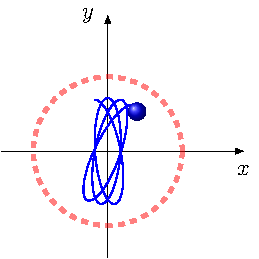
\includegraphics[height=3cm]{P1/TrajGuide_a}}
Il est important de garder à l'esprit que les atomes ne se propagent pas \emph{exactement} suivant l'axe $z$. Ils sont aussi animés d'un mouvement dans le plan transverse $(x,y)$ (voir la section~\nref{sec:MesureTempTrans}). Or nous avons vu dans la section~\nref{sec:ConfigMagnetiqueGuide} que plus la composante longitudinale $\Bpara$ est importante, plus le piège s'ouvre transversalement.
Réciproquement, plus un atome \sotosay{orbite} loin de l'axe du guide, moins il est sensible à la présence du \mima. 
%Pour s'en convaincre, il suffit de dériver le potentiel $U(r,z)$ par rapport à $z$.
% et de constater que c'est une fonction dont le module est décroissant en $r$..
%Ceci est dû au fait que le module du \chm donné par l'équation~\nref{eq:MiroirUB0} est d'autant plus sensible à la composante longitudinale ${B_0}(z)$, que la composante transverse $\gradB^2\,r^2$ est petite.
%\[
%\Diff{U(r,z)}{z} =\mu\,\Diff{\Bpara(z)}{z}\,\frac{1}{\sqrt{1+\tfrac{\gradB^2\,r^2}{\Bpara^2}}}
%\]

Il en résulte un couplage entre le mouvement transverse des atomes et le mouvement longitudinal suivant l'axe du guide.
Nous allons cependant négliger cet effet et considérer que la modélisation \emph{unidimensionnelle} est correcte.
Nous justifions ce choix par le fait que:
\begin{itemize}
	\item les fréquences d'oscillations transverses dans le \gm sont de l'ordre du kilohertz.
	\item le temps que met un atome à être réfléchi est typiquement d'un dixième de seconde (déduit de l'extension longitudinale de la barrière, $\approx \cm{6}$, et de vitesses relatives inférieures à $\vmax = \SI{1}{\meter\per\second}$).
\end{itemize} 
Les deux échelles de temps étant très différentes, il est raisonnable de négliger le couplage entre degrés de liberté transverses et longitudinal.
% (C'est une \emph{approximation séculaire}).
}

\NoteGael{PEUT ETRE FIGURE 3D\\
La figure~\nref{fig:PotentielGuideB0} montre la déformation du potentiel auquel les atomes sont soumis dans le \gm en présence du \mima.
%\bfig
%\includegraphics[width = \linewidth]{P2/PotentielGuideB0}
%\CaptionFig{fig:PotentielGuideB0}
%\label{fig:PotentielGuideB0}
%\efig
}

\vspace{5cm}

\casse

\section{Mise en mouvement du miroir} \label{sec:MiroirMiseEnMouvement}

Afin de mettre en mouvement le \mima%représenté sur la figure~\nref{fig:MiroirMontageAimant}
, nous l'avons fixé sur un \sotosay{tapis roulant} longeant le \gm. Dans la suite, ce système sera désigné par le terme \sotosay{\conv}.  Une représentation du système fait l'objet des figures~\nref{fig:MiroirConveyerSchema} et~\nref{fig:MiroirConveyerPhoto}.

\bfig
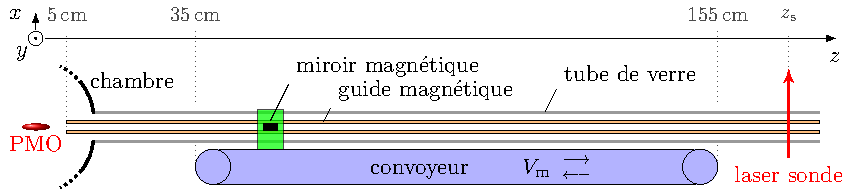
\includegraphics{P2/MiroirConveyer}
\CaptionFig{Schéma représentant le \setup du \mimamo. Celui-ci est fixé à la courroie du \conv et parcourt le rail de manière cyclique à la vitesse $\Vmir$. À chaque extrémité il subit une phase de retournement hémicirculaire. \\
Une fois injecté dans le \gm, le \pat issu du \pmo (PMO) atteint la région couverte par le \conv.  \\
Un laser sonde positionné en $z=\zsonde$ permet de mesurer la \datlin (voir la section~\nref{sec:MesureDensiteGuide}).
%En pratique, le \pmo (PMO) est protégé de par un bouclier en $\mu$-métal contre l'influence du miroir magnétique.
}
\label{fig:MiroirConveyerSchema}
\efig
\bfig
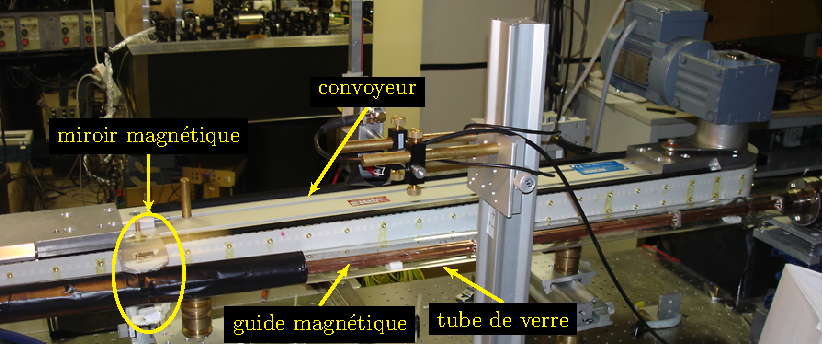
\includegraphics[width = \linewidth]{P2/MontageMiroirConveyer}
\CaptionFig{Photographie du \setup. On y distingue le \gm dans le tube de verre et le \mimo fixé sur le \conv.}
\label{fig:MiroirConveyerPhoto}
\efig

\RemarqueTitre{Accélération violente en bout de rail}{
Le fonctionnement cyclique du \conv implique que le \mimo fixé à la courroie doit subir à chaque extrémité du rail une phase de retournement hémicirculaire. 
On notera que cette accélération en bout de rail n'est pas purement centrifuge. En effet, le miroir doit résister non-seulement à une force centrifuge qui tend à l'arrachement radial du miroir, mais aussi à une force de cisaillement qui tend à faire plier le miroir autour de l'axe de rotation. 

Cette deuxième composante vient tout simplement du fait que :
\begin{itemize}
	\item sur la partie rectiligne du \conv, chaque point du miroir possède la même vitesse (celle de la courroie), 
	\item lors de la phase circulaire, les points du miroir situés loin de l'axe de rotation doivent posséder une vitesse plus importante.
\end{itemize}

En d'autres termes, cela traduit la \emph{mise en rotation} du miroir à l'instant \emph{précis} où celui-ci passe de la partie rectiligne à la partie circulaire. Cette accélération est très violente, elle est même théoriquement infinie si l'on devait considérer le système comme étant rigide. En pratique, la courroie absorbe le choc en se déformant, mais il est prudent d'assurer une bonne rigidité de fixation des aimants tout en maintenant la légèreté de l'ensemble afin d'en minimiser le moment d'inertie.
}

\subsection{Le \conv}

Le \conv a été acheté auprès de la société NORCAN. La longueur du rail est de $\cm{120}$, et la courroie de $\cm{250}$ de long qui est enroulée autour, comporte 50 emplacements de fixation (tous les \cm{5}). Le moteur électrique monté d'origine sur le système est de type asynchrone triphasé et est refroidi par un ventilateur dont l'axe est solidaire de l'arbre moteur. Il est par ailleurs contrôlé par un boîtier électronique externe fournissant le courant alternatif à la fréquence voulue, et sur lequel peuvent être programmés les différents paramètres liés au mouvement du \conv:
\begin{itemize}
	\item tension efficace appliquée au moteur,
	\item accélération au démarrage et au freinage,
	\item vitesse maximale, etc...
\end{itemize}

La liaison cinématique entre l'arbre moteur et le \conv est effectuée par un étage de démultiplication à vis sans fin de rapport $\ttfrac{1}{10}$. L'ensemble moteur est monté sur \termetech{silent-bloc} afin d'éviter les contraintes mécaniques entre le \conv et le bloc moteur.

\EnFaitNon
{
\subsection{Mesure de stabilité de la vitesse du tapis}
Une connaissance précise de la vitesse du \conv est requise pour mener à bien les expériences de \mimo. 
Aucun dispositif n'étant prévu à cet effet, nous avons installé une diode électroluminescente (LED) couplée à une photodiode dans le carénage de protection du moteur, de manière à ce que le faisceau lumineux soit coupé à chaque passage d'une des 5 palles du ventilateur (solidaire de l'arbre moteur). 
Le signal \sotosay{haché} récupéré par la photodiode nous permet de déterminer la vitesse de rotation du moteur et d'en déduire la vitesse du \conv (de manière très précise du fait de l'étage de démultiplication qui joue en notre faveur).\Cahier{8,22} \Cahier{7,35}
\picskip{0}
Nous avons ainsi pu mesurer la stabilité de la vitesse du \conv dans différentes conditions, et il s'est avéré qu'avec les réglages d'origine, la vitesse du \conv n'était pas stable à faible vitesse (en dessous de $\cmps{20}$, les fluctuations relatives de vitesse atteignaient près de $50$\%)\Cahier{7,163}. 
Grâce aux différentes possibilités de réglage offertes pas le boîtier électronique du \conv, il nous a été possible d'augmenter le couple du moteur. En contrepartie d'un échauffement accru du moteur, la stabilité en vitesse du \conv est grandement améliorée puisqu'il est possible de faire fonctionner le \conv à une vitesse de $\cmps{5}$ sans à coup (fluctuations inférieures à $10$\%).
% (la dispersion de vitesse est inférieur à $\cmps{2}$).
\Cahier{7,187 peut être encore mieux avec 8,21-22 pour la figure~\nref{fig:ConvStability} aussi.}
}

{\AjouteLigne}

\subsection{Synchronisation du mouvement avec le reste de l'expérience}

%La stabilité en vitesse du \conv dont il est question plus haut nous permet de considérer sa vitesse comme constante sur toute la durée d'une expérience de réflexion d'atome. 
Il est absolument crucial pour nos expériences de disposer d'une synchronisation parfaite du \mimo avec le lancement du \pat dans le \gm. Le mouvement du \conv est difficile à contrôler de manière dynamique du fait de l'inertie du système, d'autant plus que le boîtier électronique qui le commande n'est pas prévu pour ce genre de tâche. En revanche, tout notre dispositif expérimental de production et d'injection de \pats est piloté par un ordinateur \nomofficiel{National Instruments} qui permet, entre autres choses, de déclencher les séquences expérimentales. 

Dans le but d'assurer une bonne synchronisation, nous avons placé à proximité du \conv une sonde magnétique sensible au passage du \mimo et qui déclenche l'exécution de notre séquence. Cette dernière comporte d'ailleurs un \sotosay{temps mort}(pendant lequel rien ne se passe) réglable à volonté depuis l'ordinateur et qui permet de définir l'avance $\Zmirini$ qu'a le \mimo par rapport au \pat lors de son injection dans le \gm. 


%\casse


\section{Résultats obtenus}\label{sec:Resultats}
Les expériences réalisées dans le but de démontrer l'efficacité de cette technique seront présentées selon deux aspects complémentaires:
\begin{itemizel}
	\item expériences avec des \pats uniques afin de tester les prédictions théoriques et de démontrer l'efficacité de notre méthode de ralentissement. Elles font l'objet de la sous-section~\nref{sec:ResultatPaquetUnique}.
	\item expériences avec des \patss pour étudier le problème dans le contexte plus précis de notre expérience, \cad en vue de réaliser un \jatgm lent et ultra froid. Elles font l'objet de la sous-section~\nref{sec:ResultatPaquetMultiple} et nous amèneront à considérer les avantages de la \techmimo par rapport à l'utilisation d'une \secpent.
\end{itemizel}
Pour tous les résultats présentés ci-dessous, un courant de $\SI{200}{\ampere}$ dans chaque tube du \gm a été utilisé, générant ainsi un gradient transverse de \chm $b'=\gausspcm{500}$. 

Dans toute la suite, l'origine de l'axe $z$ du \gm est prise comme étant la position initiale du \pat (qui correspond à la position du \pmo), et le temps $t=0$ est défini par l'instant où le \pat est injecté dans le \gm. 
La détection des atomes s'effectue grâce à la technique décrite dans la section~\nref{sec:MesureDensiteGuide}. Nous pouvons de cette manière accéder à la \datlin $n(z,t)$ en $z = \zsonde = \cm{175}$ (sauf mention contraire). 

\subsection{Réflexion d'un paquet unique} \label{sec:ResultatPaquetUnique}
Chaque expérience décrite dans cette sous-section consiste en l'injection à une vitesse $\vinj$ d'un seul \pat dans le \gm. On étudie le comportement de ce paquet en présence du \mimo dont la vitesse est $\Vmir < \vinj$ et sa position à l'instant initial est $\Zmirini$.

\ifthenelse{\FormatEUE > 0}{}
{\AjouteLigne}

\subsubsection{Caractérisation du \pat avant la collision}
\label{sec:CaracPatLibre}
De manière à pouvoir étudier la réflexion sur le \mimo, il nous faut d'abord caractériser le \pat avant la réflexion. 
Pour ce faire, chaque expérience impliquant le \mimo est réalisée \emph{une deuxième fois}, à l'identique, mais \emph{sans l'intervention du \mimo}. Nous obtenons de cette manière, pour chaque expérience, un signal supplémentaire de détection correspondant à la propagation libre d'un \pat. 
%
\inlinefig{{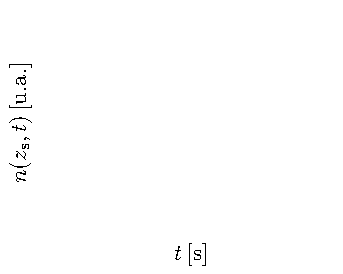
\includegraphics[scale=0.97]{P2/CourbePaquetLibre}}}%
%
De ce signal $n(\zsonde,t)$, nous déduisons les caractéristiques initiales du paquet en ajustant une fonction%
\footnote{Rappelons la formule :
$
n(\zsonde,t) = C\,\Expo{-\tfrac{m}{2\,\kb\,\Tlongini}
	\,\left( \tfrac{\zsonde}{t}-\vinj\right)^2}
$, dont les paramètres à ajuster sont la vitesse d'injection $\vinj$, la \templong $\Tlong$ ainsi que l'amplitude $C$ du signal.}
 donnée par l'équation~\nref{eq:ntPaquetAvantCol}. 
La figure ci-contre montre un exemple de signal expérimental de détection $n(\zsonde,t)$ pour un \pat typique en propagation libre. On y distingue nettement le passage du \pat devant le laser sonde, environ \seconde{1.5} après son injection. 
\picskip{3}
\noindent
En utilisant la fonction d'ajustement (dessinée en rouge), nous déduisons la vitesse d'injection $\vinj = \cmps{120}$ et la \templong $\Tlong = \microK{150}$ du \pat (cette température correspond à une \dispvitlong de \cmps{12}).
%, et pour lequel nous déduisons une vitesse moyenne de \cmps{142} ainsi qu'une \dispvitlong de \cmps{12} (correspondant à une \templong de \microK{150}).
%\bfig
%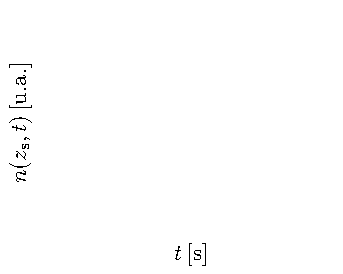
\includegraphics[width = \linewidth]{P2/CourbePaquetLibre}
%\CaptionFig{%
%On distingue sur cette figure un pic de détection aux environs de $t=\SI{1.2}{\second}$ qui traduit l'arrivée du \pat au niveau de la sonde située en $z=\zsonde = \cm{175}$. En utilisant une fonction d'ajustement de la forme de~\nref{eq:ntP..}, il est possible de déduire la vitesse d'injection $\vinj = \cmps{142}$ et la \templong $\Tlong = \microK{150}$ du \pat.}
%\label{fig:CourbePaquetLibre}
%\efig
\Remarque{
N'oublions pas que l'équation~\nref{eq:ntPaquetAvantCol} suppose que le \pat soit initialement ponctuel, alors que son extension suivant l'axe $z$ après la phase de capture dans le \pmo et de refroidissement dans la mélasse mouvante est plutôt de l'ordre de $\cm{1}$. Il est néanmoins raisonnable de négliger cette taille initiale si la \dispvitlong induit un étalement qui devient prédominant. Or, dans nos expériences, celle-ci est typiquement de l'ordre de $\cmps{10}$. Donc quelques dixièmes de seconde de propagation libre suffisent à rendre l'hypothèse raisonnable. C'est bien le cas dans toutes nos expériences.
}

\subsubsection{Caractérisation du \pat après la collision}

Fort de la connaissance des caractéristiques du \pat avant la collision, nous pouvons désormais nous concentrer sur l'étude du signal de détection $n(z,t)$ observé dans une expérience de collision avec un \mimo.

\nnRemarque{
La description d'une collision avec une barrière de potentiel ayant la forme décrite par la figure~\nref{fig:AimantPaireChampLong} est compliquée dans la mesure où le temps mis par une particule pour \sotosay{rebrousser chemin} dépend a priori de sa vitesse d'arrivée sur la barrière de potentiel. Nous avons cependant décidé d'appliquer le modèle de la barrière de potentiel infinie afin d'interpréter nos données. 

Ce choix est justifié par le fait que nos \pats possèdent une \dispvitlong relativement faible par rapport à leur vitesse moyenne (même dans le \refmir, dans lequel la collision est décrite simplement). Chaque atome met ainsi environ le même temps pour être réfléchi.
}

La figure~\nref{fig:CourbePaquetReflechi} représente le signal de détection en $z = \zsonde = \cm{175}$ en fonction du temps pour un \pat injecté à une vitesse $\vinj = \cmps{142}$ en propagation libre, puis pour un \p identiquement préparé, mais ayant subi une réflexion sur le \mimo animé d'une vitesse $\Vmir = \cmpspm{86}{2}$. 
%
\bfighs
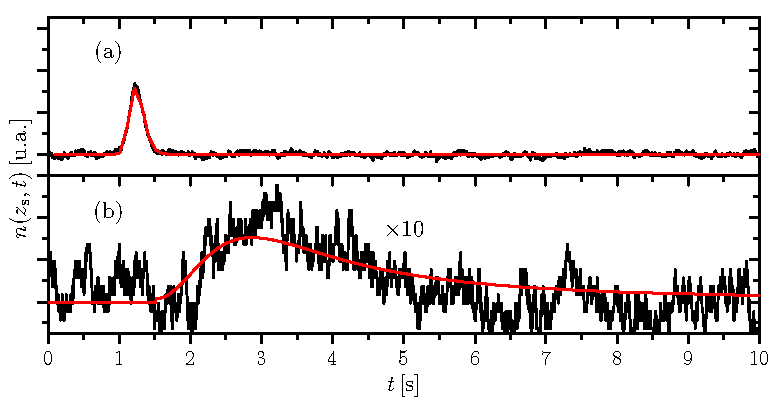
\includegraphics{P2/CourbePaquetReflechi}
\CaptionFigss{%
Signal d'absorption de la sonde donnant la \datlin $n(\zsonde, t)$ (a) pour le \pat en propagation libre. Par ajustement de la fonction~\nref{eq:ntPaquetAvantCol} (représentée en rouge), nous déduisons $\vinj = \cmps{120}$ et la \templong $\Tlong = \microK{150}$; (b) pour un \p identique, mais ayant subi une collision avec le \mimo  se déplaçant avec une vitesse $\Vmir = \cmpspm{86}{2}$. L'échelle du graphe (b) est dix fois plus précise que celle du graphe (a).
En utilisant les caractéristiques mesurées du \pat en propagation libre, nous pouvons comparer la \datlin mesurée à celle attendue en appliquant la formule~\nref{eq:NtPaquetResultat} (la courbe est tracée en rouge).}
\label{fig:CourbePaquetReflechi}
\efigh

\pagebreak

\Resultat{
La courbe expérimentale obtenue pour le \p après réflexion est compatible avec celle prévue théoriquement par l'expression~\nref{eq:NtPaquetResultat}. Le \p possède alors une vitesse moyenne $2\,\Vmir-\vinj \approx\cmps{30}$, et sa \dispvitlong est restée inchangée. Ceci signifie que son énergie cinétique a été diminuée d'environ \val{96}\%.
}


\subsection{Réflexions de \patss} \label{sec:ResultatPaquetMultiple}
Comme mentionné dans le chapitre~\nref{chap:JetAtomique} (\autoref{sec:InjectionGuide}), l'intérêt de disposer d'une méthode pour ralentir les \pats réside dans le fait que l'injection périodique dans le \gm est plus efficace (en terme de flux) si la vitesse de lancement est élevée.

Nous avons mené des expériences de principe visant à prouver la faisabilité d'un \setup optimisé pour la formation d'un jet%
\footnote{En effet, notre expérience n'ayant pas été initialement prévue pour étudier la réflexion de \pats sur un \mimo, nous n'avons pas pu jouer sur tous les paramètres qui seront décrits dans la \autoref{sec:MiroirParamPertinent}}%
. 
Pour ce faire, nous avons injecté des \pats de manière périodique dans le \gm, toujours en maintenant une bonne synchronisation de l'injection avec le mouvement du \mimo%
\footnote{en pratique, le \conv tourne en continu de manière indépendante, et c'est la \seqexp qui se déclenche périodiquement au moment idoine en fonction de la position du miroir}. En pratique, sur notre \setup, le taux de répétition pour l'injection est limité par la vitesse du miroir que nous pouvons ajuster typiquement entre \cmps{60} et \cmps{120}. La \couconv mesurant \cm{250}, nous pouvons répéter un cycle toutes les \val{2} à \seconde{4}.

\bfigss
\subfloat
{\label{fig:CourbePaquetsSuccessifs_a}
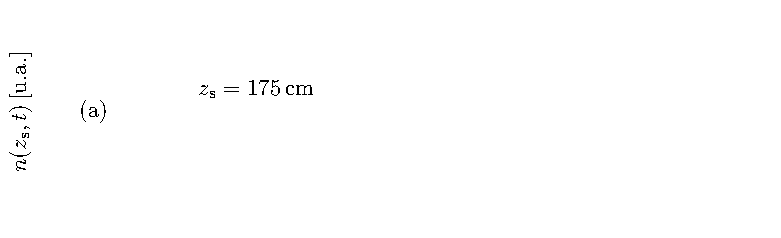
\includegraphics{P2/CourbePaquetsSuccessifs_a}}\\
\RemonteUnPeuFig
\RemonteUnPeuFig
\RemonteUnPeuFig
\subfloat
{\label{fig:CourbePaquetsSuccessifs_b}
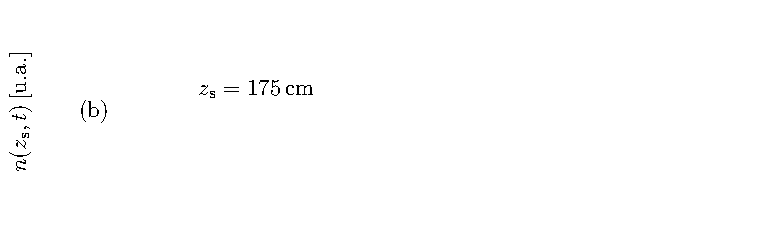
\includegraphics{P2/CourbePaquetsSuccessifs_b}}\\
\RemonteUnPeuFig
\RemonteUnPeuFig
\RemonteUnPeuFig
\subfloat
{\label{fig:CourbePaquetsSuccessifs_c}
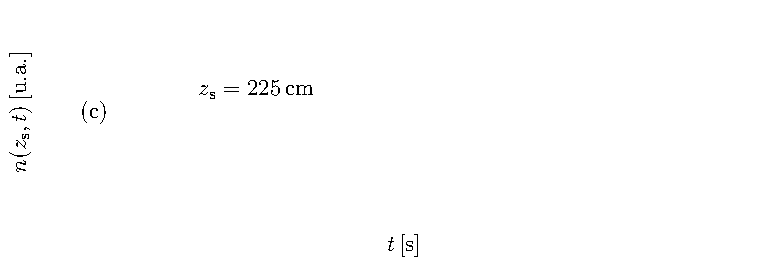
\includegraphics{P2/CourbePaquetsSuccessifs_c}}
\CaptionFigss{%
Ralentissement successifs de \pats. Les signaux d'absorption représentés donnent la \dat linéique $n(\zsonde = \cm{175}, t)$ (a) pour les \pats en propagation libre (vitesse d'injection $\vinj = \cmps{120}$); et (b), pour des \pats identiquement préparés, mais ayant chacun subi une collision avec le \mimo  se déplaçant avec une vitesse $\Vmir = \cmpspm{85}{2}$. Les \pats ont clairement été ralentis, et sont sur le point de se chevaucher. La courbe (c) correspond à une sonde positionnée plus en aval ($\zsonde = \cm{225}$) et illustre le fait que les \pats ralentis commencent bien à se chevaucher.}
\label{fig:CourbePaquetsSuccessifs}
\efig
La figure~\nref{fig:CourbePaquetsSuccessifs} correspond à un signal d'absorption $n(\zsonde, t)$ obtenu lors du ralentissement de \patss. L'injection des \ps se fait à $\vinj = \cmps{120}$, et le \mimo se déplace à $\Vmir = \cmpspm{85}{2}$.
On y voit clairement l'effet de ralentissement de chaque \pat. Cependant, leur étalement spatial n'est pas suffisant pour observer le recouvrement en $z=\zsonde=\cm{175}$. De manière à observer leur recouvrement, la même expérience est effectuée, mais en positionnant cette fois la sonde en $\zsonde=\cm{225}$ (figure~\nref{fig:CourbePaquetsSuccessifs_c}).

\subsubsection{Expériences à deux miroirs}
Pour les expériences de ralentissement successifs qui font l'objet de la figure~\nref{fig:CourbePaquetsSuccessifs}, le taux de répétition est d'environ une injection toutes les trois secondes. Nous allons voir dans la sous-section suivante qu'il serait intéressant de pouvoir ajuster le taux de répétition afin d'optimiser la \dat du jet obtenu par recouvrement des \ps.

Nous avons effectué une expérience de principe montrant qu'il est possible de doubler le taux de répétition en plaçant deux miroirs magnétiques sur la \couconv. La figure~\nref{fig:CourbePaquetsSuccessifs2Bar} représente le signal d'absorption $n(\zsonde, t)$ obtenu lors du ralentissement de \patss. 
\bfigss
\subfloat
{\label{fig:CourbePaquetsSuccessifs_2Bar}
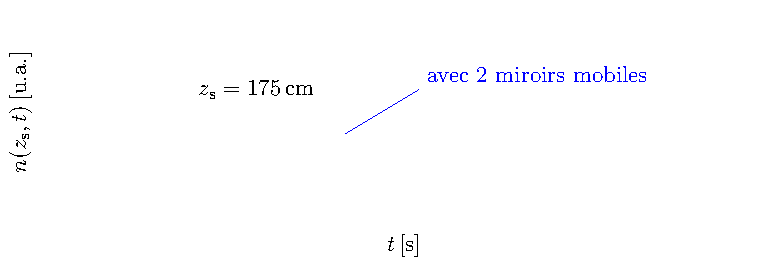
\includegraphics{P2/CourbePaquetsSuccessifs_2Bar}}
\CaptionFigss{%
Ralentissement successifs de \pats. Les signaux d'absorption représentés donnent la \dat linéique $n(\zsonde, t)$ prise dans des conditions similaires à celle qui font l'objet de la figure~\nref{fig:CourbePaquetsSuccessifs_b} , avec un \mi (courbe rouge), puis avec deux \mis (courbe bleu) fixés sur la \couconv. Nous démontrons ainsi dans le deuxième cas le ralentissement de \patss avec un taux de répétition deux fois plus élevé.}
\label{fig:CourbePaquetsSuccessifs2Bar}
\efig


\casse


\subsection{Paramètres pertinents à considérer pour la formation d'un jet}\label{sec:MiroirParamPertinent}

\subsubsection{Représentation schématique dans l'\edpup}
Le système que nous avons défini étant unidimensionnel, il est commode de représenter graphiquement son évolution sur l'espace des coordonnées $(z,v_z)$ de l'\edpup. 

\inlinefig{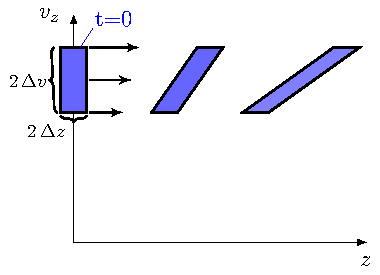
\includegraphics{P2/PhaseSpacePaquetLibre}}
La figure ci-contre montre un exemple de propagation libre d'un \pat. Pour plus de clarté, nous représenterons les \emph{paquets initiaux par des rectangles} dans l'\edpup et nous \emph{négligerons les collisions inter-atomiques}. 
Cela nous permettra de décrire les phénomènes physiques que nous voulons mettre en valeur grâce à une simplification des schémas, tout en permettant une représentation aisée des deux paramètres cruciaux en jeu:
\begin{itemize}
	\item l'extension spatiale $\DeltaZPaquet$ d'un paquet,
	\item et sa \dispvitlong $\DeltaVPaquet$.
\end{itemize}
\picskip{0}

\Remarque{
La \dispvitlong implique l'étalement spatial du \p suivant l'axe $z$.
L'inclinaison du \p dans l'\edpup traduit quant à elle les corrélations position-vitesse qui s'établissent lors de la propagation:
\begin{itemize}
	\item les atomes initialement les plus rapides vont progressivement se retrouver à l'avant du nuage ($z$ élevés).
	\item les atomes les plus lents restent à l'arrière du nuage ($z$ faibles).
\end{itemize}
}

\subsubsection{Optimisation du taux de répétition}

Intéressons nous maintenant à l'optimisation de la \techmimo en vue de la formation d'un \jat lent. Le traitement séquentiel des \ps ainsi que les contraintes sur les vitesses d'injection (liées à notre \setup) en font un problème non trivial. 

\noindent Lors du ralentissement d'un \pat, le \mimo ne doit pas interagir avec le paquet précédemment ralenti. Ceci implique notamment des contraintes sur:
\begin{itemizel}
	\item la durée $\Tcol$ de la collision entre un \pat et le \mimo,%
\nome{\Tcol}{Durée de la collision entre un \pat et le \mimo}%
	\item la longueur $\Lcol$ nécessaire pour effectuer la réflexion.%
\nome{\Lcol}{Longueur nécessaire pour effectuer la réflexion d'un \pat}%
\end{itemizel}

%\Resultat
{
Les différents paramètres à prendre en compte et qui sont récapitulés sur la figure~\nref{fig:ParamImportant} 
 sont :
\begin{itemize}
	\item \dispvitlong $\Dv$ de chaque \pat,%
\nome{\Dv}{Dispersion de vitesse longitudinale d'un \pat}%
	\item extension $\Dz$ initiale des paquets,%
\nome{\Dz}{Dispersion en position initiale d'un \pat}%
	\item vitesse $\vinj$ d'injection,
	\item distance $\Zmirini$ initiale du miroir lors de l'injection d'un paquet,
	\item vitesse $\Vmir$ du miroir,
	\item épaisseur $\EpMir$ du miroir,%
\nome{\EpMir}{Épaisseur du miroir}%
	\item période $\Trep$ de répétition d'un cycle d'injection et ralentissement.%
\nome{\Trep}{Période de répétition d'un cycle d'injection}%
\end{itemize}
}
\bfig
\RemonteUnPeuFig
\subfloat
[$t=0$: injection du \p $n$]
{\label{fig:ParamImportant_a}
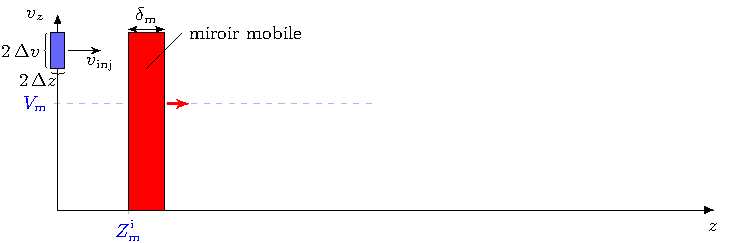
\includegraphics{P2/ParamImportant_a}}\\
\RemonteUnPeuFig
\subfloat
[$t=t_1$: début de la collision du \p $n$]
{\label{fig:ParamImportant_b}
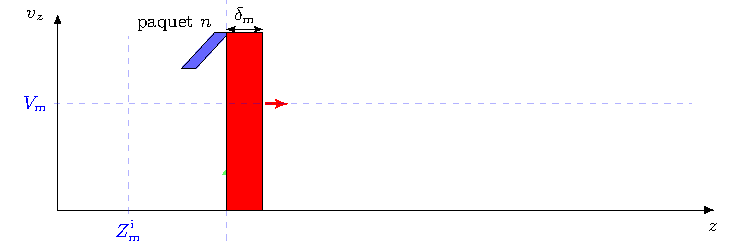
\includegraphics{P2/ParamImportant_b}}\\
\RemonteUnPeuFig
\subfloat
[$t=t_2 \equiv t_1 + \Tcol$: la collision se termine, le miroir va se repositionner]
{\label{fig:ParamImportant_c}
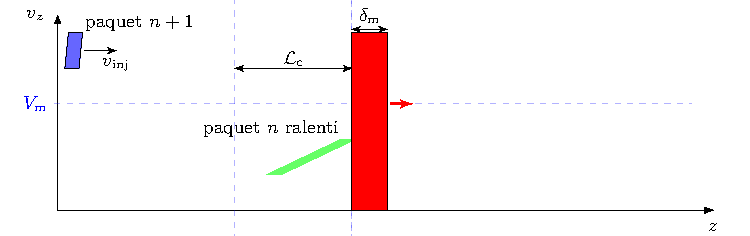
\includegraphics{P2/ParamImportant_c}}\\
\RemonteUnPeuFig
\subfloat
[$t=t_1 + \Trep + \Tcol$: fin de la collision $n+1$, le \p $n$ n'est pas affecté]
{\label{fig:ParamImportant_d}
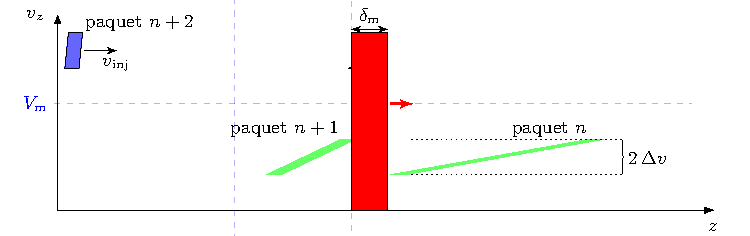
\includegraphics{P2/ParamImportant_d}}
\RemonteUnPeuFig
\CaptionFig{Succession de schémas représentant l'évolution des \pats lors de ralentissements successifs et qui correspondent à: (a) l'instant initial $t=0$ d'injection du \sotosay{paquet $n$}; (b) l'instant $t=t_1$ du début de la collision avec le \mimo; (c) l'instant $t = t_2 \equiv t_1 + \Tcol$ de la fin de la collision; (d) l'instant $t=t_1 + \Trep + \Tcol$ de la fin de la collision avec le \sotosay{paquet $n+1$}. Il faut alors que tous les atomes du \sotosay{paquet $n$} aient quitté la zone d'action du miroir. % définie par $\Lcol + \EpMir$.
On comprend l'importance de disposer d'un agencement permettant au \mi de n'agir que sur une distance donnée. 
}
\label{fig:ParamImportant}
\efig

\noindent On peut montrer que la durée $\Tcol$ et la longueur $\Lcol$ sur laquelle s'opère la collision s'expriment comme suit:
\begin{align}
	\Tcol =& 2\,\frac{\Zmirini\,\Dv + \Dz\,(\vinj-\Vmir)}{(\vinj-\Vmir)^2 - \Dv^2} 
	\nonumber \\
	\Lcol =& \Vmir\,\Tcol
	\pointformule
	\label{eq:TcolLcol}
\end{align}
La condition sur la période de répétition $\Trep$ afin que le \mimo ne \sotosay{gêne} pas le \pat précédemment ralenti peut se traduire de la manière suivante : les premiers atomes ralentis, et qui deviennent alors les plus lents (voir figure~\nref{fig:ParamImportant_a}) doivent parcourir une distance $\Lcol + \EpMir$, avant que l'arrière du miroir ne les \sotosay{rattrape}, à l'itération suivante, un temps $\Trep + \Tcol$ plus tard (voir figure~\nref{fig:ParamImportant_d}). Ceci se traduit mathématiquement par :
\[
	(\Trep + \Tcol)\,\left( 2\,\Vmir - (\vinj+\Dv) \right) \geq \Lcol + \EpMir
	\virguleformule
\] 
et implique une borne inférieure $\Trepmin$ à la période de répétition:%
\nome{\Trepmin}{Période minimale de répétition de l'injection}%
\begin{align}
	\Trep \geq \Trepmin \equiv & \frac{\Lcol + \EpMir}{2\,\Vmir - \vinj - \Dv} - \Tcol \nonumber \\
	= & \frac
	{ \EpMir\,(\vinj - \Dv - \Vmir) + 2\,\Dz\,(\vinj - \Vmir) + 2\, \Zmirini \Dv
	}
	{ (2\,\Vmir - \vinj - \Dv)\,(\vinj - \Dv - \Vmir)
	} 
	\pointformule
	\label{eq:DefTrepMin}
\end{align}

\noindent Afin de produire des flux atomiques élevés, on désire répéter l'injection d'un nouveau \p le plus souvent possible%
\footnote{En pratique cependant, nous sommes confrontés au fait que le nombre d'atomes dans chaque \p injecté dépend fortement de la cadence d'injection. Nous négligeons ici cet aspect afin de simplifier la formulation du problème de l'optimisation du flux avec la \techmimo.}%
, \cad qu'on désire minimiser la valeur $\Trepmin$.\\
Comment y parvenir ?\\
Nous allons reformuler l'équation~\nref{eq:DefTrepMin} en faisant apparaître :
\begin{itemize}
	\item la vitesse relative $\vrel \equiv \vinj - \Vmir$ entre les \ps incidents et le \mimo.
	On a bien sûr $\vrel>\Dv$, sans quoi certains atomes des \ps n'atteindraient jamais le \mi.
	\item la vitesse finale des \ps $\vfin \equiv 2\,\Vmir-\vinj$ après réflexion. Là encore, $\vfin>\Dv$, sans quoi certains atomes ralentis reviendraient en arrière.
\end{itemize} 
%

\pagebreak

\Resultat{
Nous obtenons ainsi l'expression suivante pour la période de répétition minimale~$\Trepmin$ :
\begin{equation}
\begin{cases}
\Trepmin = \frac{\EpMir}{\vfin - \Dv} + 
	\frac
	{ 2\,\Dz\,\vrel + 2\, \Zmirini \Dv	}
	{ (\vfin - \Dv)\,(\vrel - \Dv)	} 
	\\
	\vrel > \Dv
	\\
	\vfin > \Dv
\end{cases}
%	\pointformule
	\label{eq:DefTrepMinRel}
\end{equation}
Ayant pour objectif de minimiser cette période, il faut remarquer que :
\begin{itemize}
	\item la taille $\DeltaZPaquet$ et la \dispvitlong $\DeltaVPaquet$ initiales doivent évidemment être les plus faibles possibles. 
	\item le miroir doit agir très tôt après l'injection, ce qui se traduit par le fait que $\Zmirini$ doit être le plus faible possible.
	\item nous voulons produire un \jat lent par recouvrement de \ps et avoir une vitesse finale $\vfin$ assez faible, ce qui ne va pas dans le sens de diminuer $\Trepmin$. 
%En pratique, $\vfin \approx 3\,\Delta v$ est une valeur qui permet de produire un jet monocinétique, \cad dont tous les atomes vont dans la même direction.
	\item la vitesse relative $\vrel$ doit être la plus élevée possible. Cependant, nous avons vu dans la \autoref{sec:MiroirPotentielRessenti} que celle-ci est limitée par la hauteur de la \bapot magnétique produite par le \mi.
\end{itemize}
}


\section{Miroir mobile \emph{\sotosay{démoniaque}}, et \thLi}\label{sec:ThLiMiMo}

Nous allons montrer dans cette section qu'il y a un avantage certain à ralentir des \pats à l'aide de la \techmimo.%, en comparaison du résultat obtenu avec une \secpent.
Ce procédé rend en effet possible l'obtention d'un jet ayant une \ddedp plus élevée que ce que nous obtiendrions grâce à l'utilisation d'une \secpent.
Ce point sera mis en regard du \thLi et nous amènera à considérer l'action du \mimo sur les \ps comme celle d'un \termetech{démon de Maxwell} (voir l'annexe~\nref{annexe:ThLi}).

\subsection{Augmentation de la \dmdedp}\label{sec:MiroirVioleLiouville}

%Nous avons vu que le processus de ralentissement par réflexion sur le miroir n'induit \emph{aucune augmentation} de la \dispvitlong (voir section~\nref{sec:ftPaquetReflechi}).

\Remarque{%
Pour la suite, il peut être utile de définir la notion de : \\
\sotosay{\emph{\dmdedpup}} qui sera notée $\rhomoyz$.
Celle-ci correspond à la moyenne, sur l'axe $z$, de la \ddedpup pour la distribution considérée. Pourquoi s'intéresser à cette grandeur? 

Lorsque les \pats vont s'étaler longitudinalement, puis se recouvrir pour former un jet continu, la \ddedpup sera donnée par cette moyenne. 
%De même, la \datlin du jet correspondra à la densité atomique moyenne des \ps sur l'axe $z$ (C'est simplement la conseravtion du flux).
%Cette moyenne sera en fait effectuée \emph{en amont}, ou \emph{en aval} de la zone où sont ralentis les paquets, suivant que l'on considère la \fdd des paquets initiaux, ou bien celle des paquets ralentis.
}%
\nomeRemonte{\rhomoyz}{Moyenne sur l'axe $z$ de la \ddedpup}{4cm}%

\casse

\subsubsection{Propagation de \pss injectés à intervalles réguliers}
Représentons maintenant l'évolution des \patss subissant un ralentissement.
La figure~\nref{fig:MiroirPhaseSpaceReflexion} représente l'évolution de \patss dans trois cas: 
\begin{itemize}
	\item (a): propagation libre de \pats injectés à une vitesse moyenne~$\vinj$, et à intervalles temporels réguliers $\Trep$,
	\item (b): effet d'une \secpent ralentissant les \ps préparés \emph{dans les mêmes conditions} que pour (a),
	\item (c): intervention périodique du \mimo pour ralentir chaque \p, ceux-ci étant encore une fois préparés dans les même conditions que pour (a).
\end{itemize}
%
\bfigs
\subfloat
{\label{fig:EvolLibrePaquetsJet}
%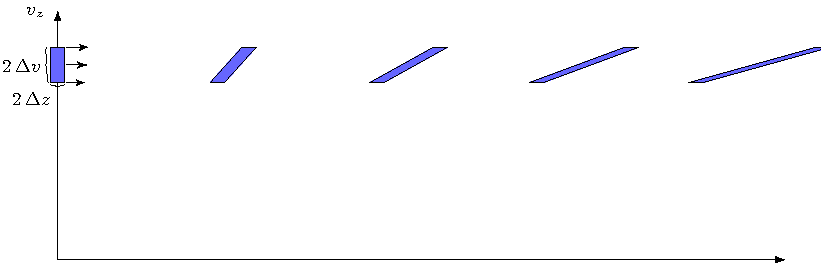
\includegraphics{P2/MiroirPhaseSpaceReflexion_a}
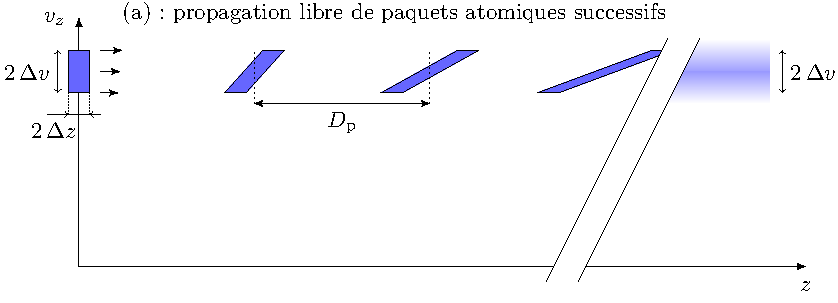
\includegraphics{P2/EvolLibrePaquetsJet}
 }\\\RemonteUnPeuFig\RemonteUnPeuFig
\subfloat
{\label{fig:EvolPentePaquetsJet}
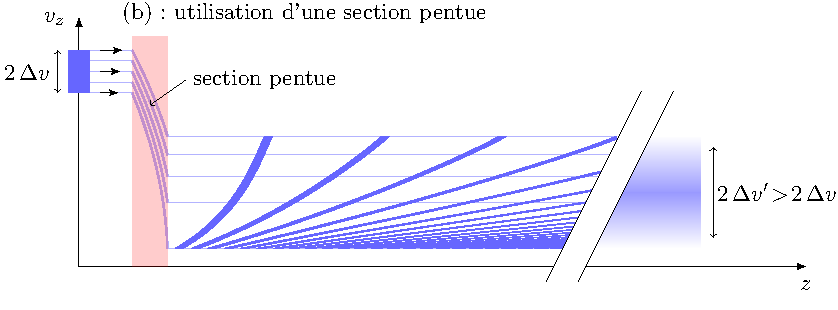
\includegraphics{P2/EvolPentePaquetsJet}
 }\\\RemonteUnPeuFig\RemonteUnPeuFig
\subfloat
{\label{fig:EvolMiroirPaquetsJet}
%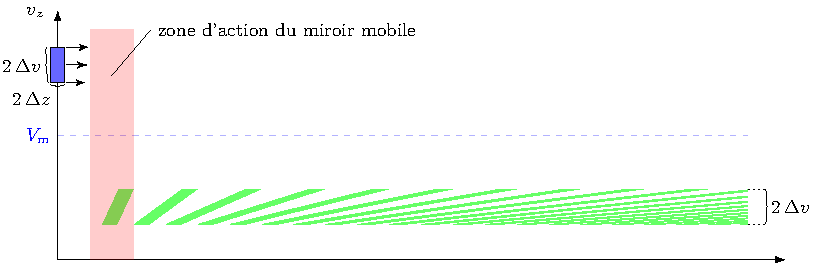
\includegraphics{P2/MiroirPhaseSpaceReflexion}
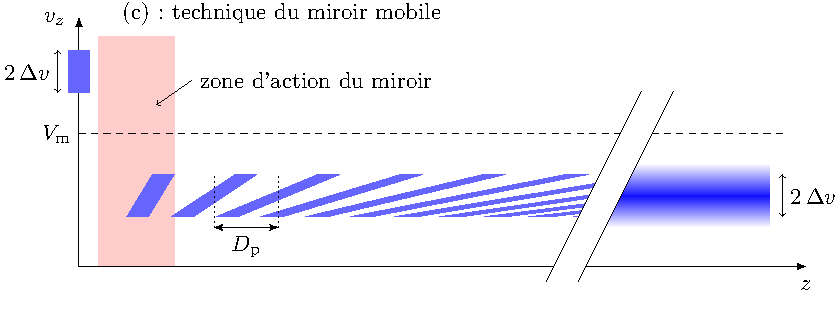
\includegraphics{P2/EvolMiroirPaquetsJet}\RemonteUnPeuFig
 }
 \RemonteUnPeuFig\RemonteUnPeuFig
\CaptionTocCaptionFig{Schématisation de l'évolution de \patss dans l'\edpup}
{Représentation de l'évolution de \patss dans l'\edpup. La partie droite des graphes représente dans chaque cas le \jat qui serait obtenu par le recouvrement des \ps et après avoir atteint un état d'\eqthdy.
\\
\vtop{\linewidth=\CaptionWidth %
\begin{itemize}
	\item (a): plusieurs \pss injectés à intervalles de temps réguliers.
	%à une vitesse $\vinj$, et à intervalles de temps réguliers $\Trep$. 
	Ces \ps sont en propagation libre. %La distance moyenne entre chaque \p est $\Trep\,\vinj$. 
	\item (b): identique à (a), mais en présence d'une \secpent qui ralentit les \ps dans le \gm. Les lignes correspondent à quelques trajectoires dans l'\edp. À cause du ralentissement, la distance moyenne entre \ps est réduite, mais on constate une nette augmentation de la \dispvitlong. Le \thLi implique que $\rhomoyz$ n'est pas plus élevée que ce qu'elle était en (a).
	\item (c): encore une fois identique à (a), mais chacun des \pss subit la réflexion sur le \mimo (voir la figure~\nref{fig:NtPaquetResultat}). La distance moyenne entre \p est réduite aussi, %devient alors $\Trep\,\left( 2\Vmir-\vinj \right)$.
mais la réflexion \emph{ne modifie pas la distribution de vitesse} des \ps. Ceci implique que $\rhomoyz$ \emph{devient plus importante} grâce au \mimo.
\end{itemize}}
}
\label{fig:MiroirPhaseSpaceReflexion}
\efig
%
%\Remarque{
%Sur la figure~\nref{fig:MiroirPhaseSpaceReflexion} on remarque que les \pats \sotosay{s'enchevêtrent} au fur et à mesure de leur propagation. Le chevauchement de plusieurs \p mène en réalité à la production d'un \jat. C'est parce que nous avons négligé les collisions inter-atomiques que les \ps restent bien séparés dans l'\edpup. Les collisions ont pour effet de gommer les corrélations position-vitesse.
%}
%Cette figure~\nref{fig:MiroirPhaseSpaceReflexion} illustre le cas de \ps injectés à intervalles réguliers $\Trep$, puis ralentis d'une vitesse moyenne $\vmoy=\vinj$ à $\vapresmoy < \vmoy$. 
Dans les cas (b) et (c), une conséquence directe du ralentissement est que la distance moyenne $\distpat$ entre les centres de masse des \ps diminue:%
(et ce quelle que soit la technique employée). En effet, par définition:
\[
 \distpat \equiv \Trep\,\vmoy
 \virguleformule
\]
où $\vmoy$ est la vitesse moyenne des \pats.
La \datlin moyenne $\nmoyz$ sur l'axe $z$ est donc plus élevée après ralentissement des atomes%
%\footnote{Ceci traduit }
:
\[
	\nmoyz \equiv \frac{\Npat}{\distpat} 
	= \frac{\Npat}{\vmoy\,\Trep}
\virguleformule
\]
$\Npat$ étant le nombre d'atomes dans chaque \p.


\subsubsection{La \dmdedpup $\rhomoyz$ peut-elle augmenter ?}
\noindent Rappelons que l'utilisation d'une \secpent impose une augmentation de la \dispvitlong ($\Dv\propto\ttfrac{1}{\vmoy}$), alors que la \techmimo la laisse inchangée.
La \dmdedpup s'exprime%
%\footnote{Dans cette expression, $m$ est la masse d'un atome.}
:
\begin{equation}
	\rhomoyz \equiv \frac{\Npat\,\hbar}{\DeltaVPaquet\,\distpat\,m} 
	= \frac{\Npat\,\hbar}{\DeltaVPaquet\,\vmoy\,\Trep\,m}
\pointformule
	\label{eq:RhoMoyZ}
\end{equation} 

\noindent On peut donc faire le constat suivant, illustré sur la figure~\nref{fig:MiroirPhaseSpaceReflexion}:
\begin{itemize}
	\item $\rhomoyz$ ne peut pas être augmentée par l'utilisation d'une \secpent,
	\[
	\rhomoypente = \rhomoylibre = \frac{\Npat\,\hbar}{\DeltaVPaquet\,\vinj\,\Trep\,m}
	\pointformule
	\]
	\item en revanche, la \techmimo augmente $\rhomoyz$ de manière évidente puisque,
\begin{align}
	\rhomoymiroir &= \frac{\Npat\,\hbar}{\DeltaVPaquet\,\left(2\Vmir-\vinj\right)\,\Trep\,m} 
	\nonumber\\
	&= \frac{\vinj}{2\Vmir-\vinj} \times \rhomoylibre
	\nonumber\\
	&> \rhomoylibre
	\pointformule
	\label{eq:RhoMiroirPlusGrand}
\end{align}	
\end{itemize}
Dans la suite, nous allègerons les notations en prenant : $\rhomoym\equiv\rhomoymiroir$.%
\nome{\rhomoym}{Densité moyenne dans l'\edp après action du \mimo}%

\Resultat{
Ceci signifie que, utilisant la \techmimo, le \jat qui sera obtenu après recouvrement des \ps aura une \ddedpup plus élevée que celle d'un jet qui aurait été obtenu avec des \ps non ralentis, ou même que celle d'un jet ralenti par une \secpent.
}

\subsection{Miroir mobile \emph{\sotosay{démoniaque}}}

La conclusion ci-dessus peut paraître surprenante au premier abord :
le \thLi n'implique-t-il pas une conservation de la \ddedpup en toute situation ?  Précisément non. L'annexe \vref{annexe:ThLi} présente l'énoncé du \thLi. Celui-ci permet de comprendre pourquoi cette technique permet d'augmenter la \ddedpup.
En effet, afin d'agir sur les \patss, le \mimo \emph{\sotosay{utilise} une information} sur la distribution initiale des atomes, à savoir:
\begin{itemize}
	\item une information sur la distribution des vitesses,
	\item mais aussi, \emph{et surtout}, une information sur la distribution en \ps distincts injectés à des instants connus.
\end{itemize}
%
%\RemonteUneLigne
%
\Resultat{
Le \mimo \sotosay{agit} comme un \emph{démon de Maxwell} (voir l'annexe~\nref{annexe:ThLi}). Nous pouvons d'ailleurs exprimer la limite absolue de cette technique quant à la \ddedpup du jet ainsi formé. 
Le miroir n'utilisant pas une information à l'échelle microscopique, \cad sur les atomes individuels, il sera impossible de dépasser la densité initiale $\rhomoyp$ d'un \pat:\vspace{-10pt}
\[
	\rhomoym
	<  \rhomoyp
	\equiv  \frac{\Npat\,\hbar}{\DeltaZPaquet\,\DeltaVPaquet\,m}
\pointformule
\]
\finformule
}%
\nomeRemonte{\rhomoyp}{Densité initiale d'un \pat dans l'\edpup}{2cm}%
%
%\AjouteLigne
%\RemonteUneLigne
%\RemonteUneLigne
\RemonteUneLigne
%
\subsection{Optimisation de la vitesse du \mi}
%
Dans cette sous-section, nous discutons de l'optimisation de la \techmimo. Nous nous proposons de calculer la vitesse optimale $\Vmiropt$ %
\nome{\Vmiropt}{Vitesse optimale du \mimo pour maximiser le rapport $\Rmax$}%
qui, pour une situation expérimentale donnée, va maximiser le rapport :
\begin{equation}
	\Rmax \equiv \dfrac{\rhomoym}{\rhomoyp} 
%	= \dfrac{
%	\frac{\Npat\,\hbar}{\DeltaVPaquet\,\left(2\Vmir-\vinj\right)\,\Trepmin\,m} }
%	{\frac{\Npat\,\hbar}{\DeltaZPaquet\,\DeltaVPaquet\,m}}
	=\frac{\DeltaZPaquet}{\left(2\Vmir-\vinj\right)\,\Trepmin}
	\virguleformule
	\label{eq:Rmax}
\end{equation}%
\nome{\Rmax}{Rapport de la \ddedp du jet et d'un \p}%
où nous avons utilisée l'expression~\nref{eq:RhoMiroirPlusGrand} en supposant que le taux de répétition de l'injection est optimale, \cad que $\Trep=\Trepmin$ (voir l'équation~\nref{eq:DefTrepMinRel}). 

\subsubsection{Cas d'un miroir d'épaisseur nulle agissant dès l'injection}
\inlinefig{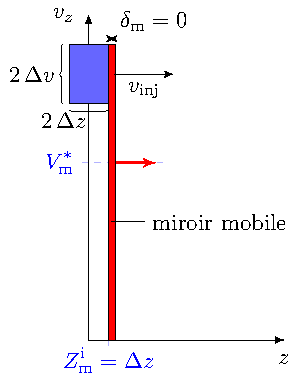
\includegraphics{P2/MiroirRmaxCasSimple}}
Afin de simplifier le raisonnement nous allons nous placer dans un cas précis pour lequel nous supposerons (voir l'illustration ci-contre):
\begin{itemize}
	\item que l'épaisseur du miroir est nulle, $\EpMir=0$,
	\item que le miroir agit sur les \ps dès leur injection. \\ En d'autres termes, le miroir est supposé au contact du \\\p à l'instant $t=0$, ce qui se traduit par $\Zmirini=\Dz$.
\end{itemize}
L'expression~\nref{eq:Rmax} peut alors se mettre sous la forme suivante, ne faisant intervenir que des grandeurs adimensionnées:
\begin{equation}
%\begin{cases}
\Rmax(x,y) = 
\frac{ \left( 2\,x-y-1 \right)  \left( x+y-1 \right) }{ \left( x
-y-1 \right)  \left( 2\,x-1 \right) }\\
\virguleformule
	\label{eq:RmaxSimple}
\end{equation}
où $x\equiv \ttfrac{\Vmir}{\vinj}$ et $y\equiv \ttfrac{\Dv}{\vinj}$. 
%\picskip{0}

\casse

\noindent
La vitesse optimale $\Vmiropt$ du miroir est obtenue en résolvant l'équation $\frac{\partial \Rmax}{\partial x}=0$ :
\begin{equation}
	\Vmiropt \equiv x^\ast \, \vinj = \vinj\,\frac{1+y+\sqrt {1-y-2\,y^{2}}}{3}
	\virguleformule
	\label{eq:VmirOpt}
\end{equation}
dont le domaine de validité est $0<y<\frac{1}{3}$.

Comme le montre la figure~\nref{fig:Xetoile}, une propriété remarquable de l'expression~\nref{eq:VmirOpt} est que $\Vmiropt$ est quasiment constante sur tout le domaine de validité%
\footnote{Les variations relative de $\Vmiropt$ sur le domaine $0<y<\frac{1}{3}$ sont inférieure à \val{3}\%.}.% et est approximativement égale à $\ttfrac{\vinj\,2}{3}$. 
\bfighss
\subfloat[]{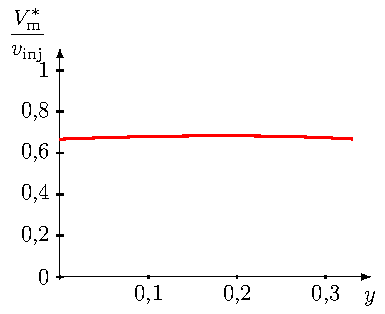
\includegraphics{P2/MiroirXetoile}\label{fig:Xetoile}}
\,\,
\subfloat[]{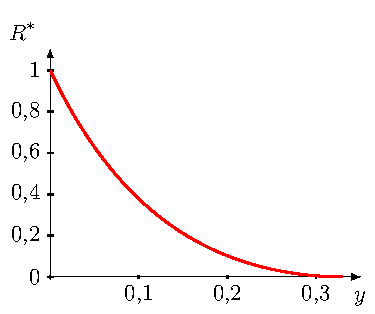
\includegraphics{P2/MiroirRetoile}\label{fig:Retoile}}
\CaptionFigs{Représentation des quantités adimensionnées $x^\ast\equiv\ttfrac{\Vmiropt}{\vinj}$ et $\Rmax^\ast\equiv\Rmax(x^\ast,y)$ en fontion de $y\equiv \ttfrac{\Dv}{\vinj}$.
$x^\ast$ est quasiment constante sur tout le domaine de validité $[0;\tfrac{1}{3}]$ et approximativement égale à $\tfrac{2}{3}$.
On voit que $\Rmax^\ast\rightarrow1$ quand $y$ tend vers 0, \cad que l'on peut atteindre la limite $\rhomoym = \rhomoyp$ si la \dispvitlong des \pats est très inférieure à la vitesse d'injection.
}
\efigh

\Resultat{
Quelles que soient les conditions expérimentales, la vitesse du miroir devra donc toujours être ajustée à la valeur :\vspace{-10pt}
\[
\Vmiropt \approx \frac{2}{3} \, \vinj 
\pointformule
\]
\finformule
}
Dans ces conditions, le rapport $\Rmax^\ast(y) \equiv \Rmax(x^\ast,y)$, est une fonction qui tend vers 1 quand $y$ tend vers 0 (voir la figure~\nref{fig:Retoile}). 
On peut donc s'approcher de la limite $\rhomoym = \rhomoyp$ si la \dispvitlong des \pats est très inférieure à la vitesse d'injection. 
Cette situation limite correspond à ralentissement instantané de chaque \p de manière à les positionner les uns contres les autres après le ralentissement.

\NoteGael{ A FAIRE PEUT ETRE UN JOUR :

Calcul de ce qu'on peut faire avec un miroir uniformément accéléré (ralenti?)
}

\casse

\subsubsection{Cas d'un miroir d'épaisseur nulle agissant après l'injection}
\inlinefig{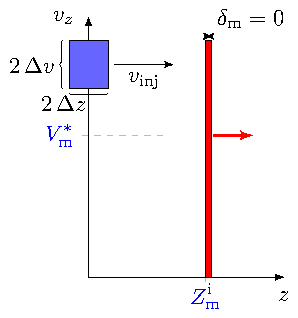
\includegraphics{P2/MiroirRmaxCasPropag}}
Si nous considérons cette fois-ci le cas d'un miroir d'épaisseur nulle, mais agissant sur le \p après que celui-ci se soit propagé librement sur une distance $D$ (voir l'illustration ci-contre), on peut montrer que l'expression~\nref{eq:RmaxSimple} devient:
\[
\Rmax'(x,y,D) = \frac{\Rmax\xy}{1+y\,\frac{D}{\Dz}}
\pointformule
\]
L'expression de $\Vmiropt$ reste donc inchangée%
\footnote{La dérivation $\ttfrac{\partial\Rmax'(x,y,D)}{\partial x} = 0$ est en effet équivalente à  $\ttfrac{\partial\Rmax(x,y)}{\partial x} = 0$.}
 et la courbe $\Rmax'^\ast$ conserve la même allure que sur la figure~\nref{fig:Retoile}.
On peut interpréter cette expression aisément : le terme au dénominateur traduit simplement le fait que le \p s'est étalé spatialement. 
\picskip{1}
%\vspace{5pt} 
\noindent En effet, on peut mettre ce terme sous la forme:
\[
1+y\,\dfrac{D}{\Dz} = \dfrac{\Dz + \Dv\,t'}{\Dz} = \dfrac{\Dz'}{\Dz}
\virguleformule
\]
où $t'$ est le temps de propagation libre, $t'=\ttfrac{D}{\vinj}$ et $\Dz'$ est donc la taille du \p au début de la réflexion. On est ainsi ramené à la même situation que précédemment, mais en considérant un \p initialement plus étalé.

\subsubsection{Cas d'un miroir d'épaisseur non nulle agissant dès l'injection}
\inlinefig{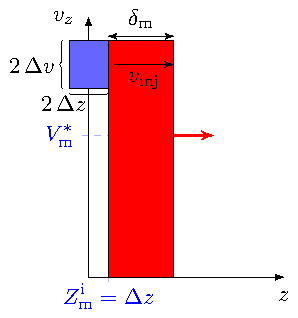
\includegraphics{P2/MiroirRmaxCasEpais}}
Considérons enfin le cas d'un miroir dont on ne néglige pas l'épaisseur $\EpMir$, mais en supposant qu'il agisse sur les \ps dès leur injection, \cad $\Zmirini=\Dz$ (voir l'illustration ci-contre). On peut montrer que la vitesse optimale $\Vmiropt$ du miroir est alors supérieure à $\tfrac{2}{3}\,\vinj$ et que la valeur maximale de $\Rmax^\ast(y)$ quand $y\rightarrow0$ est :
\[
\Avec{\Rmax^\ast}{\EpMir\neq0} = \frac{1}{1+\dfrac{\EpMir}{\DeltaZPaquet}} < 1
\pointformule
\]
On comprend la signification physique de cette expression : le miroir ayant une épaisseur non-nulle, il est impossible, même dans les meilleures conditions ($y\ll1$), de placer un \pat à moins de $\EpMir$ du \p précédemment ralenti.
\picskip{1}

\casse

\subsection{Conclusion}
Dans ce chapitre, nous avons décrit la mise en \oe uvre d'une technique de ralentissement des \pats par réflexion sur un \mimamo. Nous avons observé le ralentissement de \pats individuels ainsi que d'une succession de \ps qui, se recouvrant par la suite, forment un \j continu et très lent. Les limites des performances observée en terme de \fat sont pour l'instant dues au fait que notre \setup n'avait pas initialement été prévu pour effectuer cette tâche.

Nous avons souligné les paramètres importants à considérer afin de pouvoir, dans le futur,  concevoir une nouvelle expérience qui serait optimisée pour tirer pleinement partie des qualités de cette technique. En effet, nous avons constaté que :
\begin{itemizel}
	\item le ralentissement par réflexion n'augmente pas la \dispvitlong des \pats, contrairement à l'utilisation d'une \secpent (voir le chapitre~\nref{chap:JetAtomique}),
	\item la \ddedpup du jet ainsi formé peut être supérieure à celle obtenue en l'absence de ralentissement, ou même à celle obtenue par l'utilisation d'une \secpent.
\end{itemizel}
Ce dernier point est remarquable et nous a amené à considérer l'action du \mimo sur les \ps comme celle d'un \termetech{démon de Maxwell} (voir l'annexe~\nref{annexe:ThLi}).





%En utilisant les notations de la section~\nref{sec:MiroirParamPertinent}, nous pouvons définir l'entropie d'un système composé d'un nombre $n$ de \pats ayant une extension spatiale $\DeltaZPaquet$ et une \dispvitlong $\DeltaVPaquet$:
%%\picskip{3}
%\[
%S = n \times \Npat\,\Ln{n\,\Dz\,\Dv\,\frac{m}{\hbar}}
%\virguleformule
%\]
%où $\Npat$ est le nombre d'atomes dans chaque \p. Cette expression correspond à $n$ fois l'entropie d'un \p, à ceci près qu'on ne sait pas a priori dans quel \p se trouve un atome donné, d'où le facteur $n$ dans le logarithme $\Ln{\cdots}$.
%%\footnote{En effet, l'entropie est une grandeur extensive.}.
%
%%
%%
%\noindent En s'étalant, puis en se recouvrant, les \ps vont se mélanger pour former un \jat. La \dispvitlong du jet sera identique à celle des \ps initiaux (par conservation de l'énergie). Les deux figures ci-contre représentent les \ps s'étalant, puis, ayant formé le \jat.%
%%\picskip{0}
%%
%%\inlinefig{\fbox{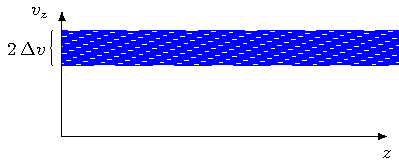
\includegraphics{P2/EntropiePaquetsJet}}}
%%
%Connaissant l'espacement $\distpat$ entre les centres de masses de deux \ps consécutifs, nous pouvons exprimer l'entropie du jet formé par le recouvrement de $n$ \ps:
%\begin{equation}
%S = n\, \Npat\, \Ln{n\,\frac{\distpat}{2}\,\Dv\frac{m}{\hbar}}
%\pointformule
%	\label{eq:EntropieJet}
%\end{equation}
%Cette expression traduit le fait qu'un atome donné peut alors se trouver n'importe où dans le jet dont la longueur considérée ici est $n\,\distpat > n\,\DeltaZPaquet$.
%L'entropie a naturellement augmenté lors de la formation du jet (c'est un phénomène irréversible). %, et atteint une valeur qui correspond à une \ddedp
%%un volume $\Omega$ plus grand dans l'\edpNp. 
%%\picskip{0}
%%
%%
%
%%\inlinefig{\fbox{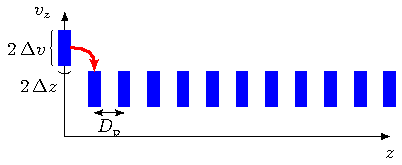
\includegraphics{P2/EntropiePaquetsMiroir}}}


%\section{Miroir mobile avec beaucoup de collisions entre atomes}
%
%Et aussi 
%
%ouverture sur une trajectoire du miroir exploitant non seulement l'information \sotosay{vitesse et position du \pat}, mais aussi l'information \sotosay{corrélation position vitesse}.
%
%par exemple, un miroir qui ralenti lors de la collision va beaucoup ralentir les atomes rapides (a l'avant du paquet) et peu les atomes lents (à la traine du paquet)...
%
%= focalistion 
%
%-> Vitesse miroir pour focaliser dans l'espace des vitesse
%
%-> Forme barrière pour focaliser dans l'espace des position (mais la \dispvitlong reste inchangée)

